\documentclass[11pt, a4paper]{article} % RULE: A4, standard font size 11

% --- EUROC MANDATORY FORMATTING PACKAGES ---
\usepackage[margin=2.5cm]{geometry} % RULE: standard page margins 2,5 cm
\usepackage{setspace}
\singlespacing % RULE: line spacing 1,0

% 1. Paquete de colores con soporte para tablas (imprescindible [table])
% OJO: Si ya tienes puesto \usepackage{xcolor}, cámbialo por este:
\usepackage[table,dvipsnames]{xcolor}

% 2. Paquetes necesarios para tablas ajustadas y multilínea
\usepackage{tabularx}
\usepackage{array}
\usepackage{booktabs}

% 3. Definición de los colores corporativos de la tabla
\definecolor{EtseNavy}{HTML}{002F6C}      % Azul marino institucional
\definecolor{LightGrayTable}{HTML}{F2F4F7} % Gris claro para filas alternas

% --- STANDARD ENGINEERING PACKAGES ---
\usepackage[utf8]{inputenc}
\usepackage[T1]{fontenc}
\usepackage{lmodern}
\usepackage{graphicx}
\usepackage{xcolor}
\usepackage{tabularx}
\usepackage{booktabs}
\usepackage{float}
\usepackage{hyperref}
\usepackage{longtable}
\usepackage{amsmath}
\usepackage{subcaption}


\usepackage{tikz}
\usetikzlibrary{arrows.meta, positioning}
\usepackage{seqsplit}

\hypersetup{
    colorlinks=true,
    linkcolor=EtseNavy,
    urlcolor=EtseNavy,
    citecolor=EtseNavy
}
% Definición del color si no lo tienes ya:
\definecolor{EtseNavy}{HTML}{002F6C}
% Comando para citar requisitos (solo el nombre del requisito va en azul marino):
\newcommand{\req}[1]{[\textcolor{EtseNavy}{\textbf{#1}}]}

% --- TITLE PAGE CONFIGURATION ---
\title{
    \vspace{-2cm}
    \includegraphics[height=3cm]{example-image} % PLACEHOLDER FOR COHETEROS LOGO
    \\[1.5cm]
    \textbf{\Huge PROJECT NAOS EVO} \\[0.5cm]
    \Large \textit{Design, Development, and Flight Readiness Status} \\[1.5cm]
    % EUROC MANDATORY SUBTITLE RULE:
    \textbf{\Large Team 07 Technical Report to the 2026 EuRoC}
}
\author{
    \textbf{Coheteros} \\ 
    Rocketry Association \\ 
    School of Engineering \\ 
    University of Seville
}
\date{August 2026} % Update to your submission date

\begin{document}

\maketitle
\thispagestyle{empty}
\newpage

\tableofcontents
\newpage

% =========================================================================
% 0. ABSTRACT (Rule: Force section numbering to start at 0)
% =========================================================================
\setcounter{section}{-1}
\section{Abstract} \textcolor{red}{actualizar con datos finales en base a lo puesto en los subsistemas}
\label{sec:abstract}

This Technical Report presents the engineering design, manufacturing qualification, and flight readiness status of NAOS EVO, a single-stage sounding rocket developed by the student association Coheteros from the Escuela Técnica Superior de Ingeniería (ETSI) at the Universidad de Sevilla. The vehicle is engineered to compete in the 3000\,m Above Ground Level (AGL) Solid Student Researched and Developed (SRAD) flight category at the 2026 European Rocketry Challenge (EuRoC). With an overall longitudinal length of 2192\,mm, an outer airframe diameter of 91\,mm, and a total lift-off wet mass of \textcolor{red}{10.86\,kg}, NAOS EVO serves as an empirical flight test bench to validate in-house multidisciplinary modeling tools against real-world aerodynamic, structural, and ballistic data.

Propulsion is delivered by a proprietary SRAD solid rocket motor operating on an Ammonium Perchlorate Composite Propellant (APCP) formulation with an HTPB binder matrix. The internal ballistics configuration incorporates six BATES propellant grains and a 14\,mm throat diameter graphite nozzle within an AISI 304 stainless steel combustion casing. Thermal protection is provided by an internal cellular polypropylene liner, validated via static fire testing. Operating at a nominal chamber pressure of 59\,bar, the motor delivers a maximum thrust of 1287\,N and a total impulse of 3521\,Ns over a 3.05\,s burn duration, establishing an initial static stability margin of 3.24\,calibres off the launch rail.

To achieve exact apogee targeting, NAOS EVO features an active aerodynamic flight control subsystem comprising four radial airbrake petals machined from 7075-T6 aluminium. Actuated by a high-torque servomotor via a slider-crank linkage, the control loop engages at 1500\,m AGL during the unpowered coast phase, utilizing an analytical root-finding guidance algorithm and an Error-State Kalman Filter (ESKF) running on an STM32H7 microcontroller. Terminal recovery is executed through a dual-stage descent architecture. Initial apogee separation is commanded by an explosive-free, cold-gas $\text{CO}_2$ pressurisation mechanism that deploys a 0.77\,m hemispherical drogue parachute. At 450\,m AGL, a pyrotechnic tender-descender cord-cutter releases the extraction bulkhead to deploy a 1.85\,m ringsail main parachute, ensuring a nominal touchdown velocity of 9\,m/s.

The onboard electronics suite comprises custom-developed printed circuit boards partitioned across three isolated power domains, integrating 868\,MHz LoRa telemetry, high-rate inertial logging, and a hardware-watchdog fail-safe interface. To satisfy EuRoC flight safety requirements, primary processing redundancy is established in hot-standby, alongside an independent commercial CATS Vega flight computer governing secondary recovery deployment. The vehicle carries a 1\,kg non-deployable dummy CanSat payload strictly adhering to competition geometric and mass criteria. NAOS EVO embodies the association's commitment to self-reliant engineering, successfully bridging academic aerospace theory with flight-proven hardware.

\vspace{0.6cm}
\noindent\textbf{Keywords:} vehicle description, mission, flight category, design characteristics, payload, special features.

\newpage

% =========================================================================
% 1. INTRODUCTION
% =========================================================================
% =========================================================================
% 1. INTRODUCTION
% =========================================================================
\section{Introduction}
\label{sec:introduction}

\subsection{Academic Programme and Institutional Framework}
Project NAOS EVO is an experimental sounding rocket programme conceived, engineered, and operated by \textit{Coheteros}, the student rocketry association based at the Escuela Técnica Superior de Ingeniería (ETSI) of the Universidad de Sevilla. The initiative operates under the university's institutional framework of \textit{Proyectos Multidisciplinares Formativos}, which fosters multidisciplinary project-based engineering education. Academic governance, institutional compliance, and safety oversight are supervised by the designated Faculty Advisor, Dr.~Francisco Rafael Gavilán Jiménez. 

The association integrates over 50 active undergraduate and postgraduate students from diverse fields, primarily Aerospace, Mechanical, Electrical, Telecommunications, Software, and Materials Engineering, supplemented by Physics, Chemistry, and Industrial Design. NAOS EVO serves as the flagship single-stage launch vehicle developed to compete in the 3000\,m Above Ground Level (AGL) Solid Student Researched and Developed (SRAD) category at the 2026 European Rocketry Challenge (EuRoC).

\subsection{Team Structure and Systems Engineering Management}
To ensure deterministic configuration control and strict adherence to the EuRoC System Requirements Document (SRD), the project enforces a formal departmental hierarchy overseen by an Executive Board (\textit{Junta Directiva}) and a Technical Direction. The technical workload is operationalized into ten specialized, requirements-driven Engineering Committees, each led by a dedicated Committee Lead:

\begin{itemize}
    \item \textbf{Motor \& Combustion Chamber Committee:} APCP solid propellant casting, cellular polypropylene liner thermal protection, nozzle geometry optimization, and hydrostatic chamber testing.
    \item \textbf{Recovery System Committee:} Dual-stage descent sizing, cross main canopy aerodynamics, line load rating, and clean-gas $\text{CO}_2$ mechanical separation.
    \item \textbf{Active Control Committee:} Structural, kinematic, and finite-element validation of the 4-petal radial airbrake mechanism and linear rail guides.
    \item \textbf{Avionics Bay Committee:} Stacked PCB layout, multi-sensor integration, isolated power domains, and COTS CATS Vega backup installation.
    \item \textbf{Airframe \& Integration Committee:} Composite airframe wet layups, Von Kármán nosecone manufacturing, fin-can assembly, and structural joint tolerances.
    \item \textbf{Missionization \& Simulation Committee:} Six-Degree-of-Freedom (6-DOF) trajectory calculation, dispersion ellipses, and rail-clearing dynamics.
    \item \textbf{Communication \& Ground Station Committee:} 868\,MHz LoRa telemetry protocols, antenna tracking systems, and real-time mission control software.
    \item \textbf{Test Bench Committee:} Instrumentation, load-cell calibration, and data acquisition architectures for static hot-fire campaigns.
    \item \textbf{Launchpad Committee:} Mechanical integration with the competition launch rail, umbilical routing, and physical safety interlocks.
    \item \textbf{Payload Committee:} Geometric, electrical, and mass compliance verification of the standardized 1\,kg dummy CanSat experiment.
\end{itemize}

Operational reporting follows a structured chain of responsibility: \textit{Task Members $\rightarrow$ Committee Leads $\rightarrow$ Technical Direction $\rightarrow$ Faculty Advisor}. Quality gates are enforced through bi-weekly interdepartmental tracking sessions and formal milestone reviews (Preliminary, Critical, and Flight Readiness Reviews).

\newpage % Salto deliberado para dar inicio a la segunda página de forma equilibrada

\subsection{Project Vision and Long-Term Roadmap}
Project NAOS EVO constitutes the baseline operational milestone of \textit{Programa ZENIT}, a multi-phase strategic roadmap established by Coheteros to progressively master sounding rocket technologies. Technical maturation is implemented through incremental validation gates; prior to NAOS EVO integration, a subscale demonstrator (\textit{BETELGEUSE}) was successfully tested to qualify core avionics, telemetry links, and recovery concepts. The association enforces a strict 100\% SRAD development philosophy, eliminating black-box commercial systems in favor of in-house physics modeling and empirical software tool development.

\subsection{Stakeholders, Industrial Partnerships, and Suppliers}
To bridge university laboratory resources with aerospace industrial standards, Coheteros collaborates with an extensive network of institutional stakeholders, technical sponsors, and specialized manufacturing contractors. Table~\ref{tab:sponsors_partners} outlines the institutional and industrial ecosystem supporting Project NAOS EVO.

\begin{table}[H]
\centering
\caption{Institutional stakeholders, industrial partners, and technical sponsors.}
\label{tab:sponsors_partners}
\renewcommand{\arraystretch}{1.2}
\begin{tabularx}{\textwidth}{|>{\raggedright\arraybackslash}p{4.2cm}|>{\raggedright\arraybackslash}p{3.8cm}|X|}
\hline
\rowcolor{EtseNavy}
\textbf{\textcolor{white}{Entity / Organization}} & \textbf{\textcolor{white}{Domain / Sector}} & \textbf{\textcolor{white}{Contribution to NAOS EVO}} \\ \hline
\textbf{Agencia Espacial Española (AEE)} & National Space Agency & Institutional patronage and aerospace ecosystem integration. \\ \hline
\rowcolor{LightGrayTable}
\textbf{ETSI (Universidad de Sevilla)} & Academic Institution & Primary institutional sponsorship, testing facilities, and laboratories. \\ \hline
\textbf{AERTEC Solutions} & Aerospace \& Defense & Technical mentorship, systems engineering, and industrial sponsorship. \\ \hline
\rowcolor{LightGrayTable}
\textbf{Solar MEMS Technologies S.L.} & Space Technologies & High-reliability aerospace systems and sensor integration support. \\ \hline
\textbf{Kistler Group} & Dynamic Measurement & High-precision piezoelectric pressure transducers and load cells. \\ \hline
\rowcolor{LightGrayTable}
\textbf{Dewesoft} & Data Acquisition (DAQ) & Advanced multi-channel DAQ hardware and test bench software. \\ \hline
\textbf{Grupo Álava (Álava Ingenieros)} & Testing \& Sensing & Specialized instrumentation, sensor solutions, and technical advisory. \\ \hline
\rowcolor{LightGrayTable}
\textbf{Mec. y Matricería Matrisur S.L.} & Precision Machining & High-tolerance CNC lathe machining of stainless steel motor parts. \\ \hline
\textbf{norelem (norelem Ibérica S.L.)} & Mechanical Engineering & Standard mechanical machine elements, fasteners, and linear components. \\ \hline
\rowcolor{LightGrayTable}
\textbf{Casemedia Embalajes S.L.} & Technical Packaging & Custom flight cases and specialized protective ground logistics containers. \\ \hline
\textbf{Dronetools S.L.} & Unmanned Aerial Systems & Advanced composite airframe manufacturing and structural tooling support. \\ \hline
\rowcolor{LightGrayTable}
\textbf{Metadev S.L.} & Software Engineering & Model-driven software architecture, tooling, and critical code reviews. \\ \hline
\textbf{Al Andalus Innovation Venture} & Innovation \& Investment & Venture ecosystem networking, entrepreneurship, and open innovation. \\ \hline
\rowcolor{LightGrayTable}
\textbf{espacio\_RES} & Startup Incubation & Strategic business acceleration and collaborative workspace facilities. \\ \hline
\textbf{AstroEmociones} & STEM Dissemination & Scientific communication, astronomy outreach, and media broadcasting. \\ \hline
\end{tabularx}
\end{table}

\subsection{Major Technical Challenges}
The qualification of NAOS EVO entails three defining engineering challenges addressed in this report:
\begin{enumerate}[noitemsep, topsep=1pt]
    \item \textbf{Proprietary Solid Propulsion Certification:} Formulating and casting a reliable composite propellant (APCP) grain with reproducible burn rates, thermally shielded by a cellular polypropylene liner inside an AISI 304 stainless steel casing operating at 59\,bar.
    \item \textbf{Closed-Loop Aerodynamic Energy Regulation:} Developing and validating an analytical guidance algorithm paired with an Error-State Kalman Filter (ESKF) to modulate airbrake drag at 1500\,m AGL without inducing destabilizing aerodynamic roll moments.
    \item \textbf{Clean-Gas Dual Recovery Deployment:} Implementing a cold-gas $\text{CO}_2$ puncture mechanism to reliably detach the ogive at apogee, paired with a staged tender-descender cord-cutter to prevent high-velocity canopy entanglement.
\end{enumerate}


% RULE: Academic program, stakeholders, team structure, management strategies, vision, suppliers/partners, technical challenges.
% INTEGRATION NOTE: Here we will add the new "departmental team structure" decided in the meeting to look more professional than just a "committee".

\vspace{0.5cm}
\noindent\textbf{Keywords:} academic programme, stakeholders, team, experience, vision, strategy, suppliers, partners, technical challenges.

% =========================================================================
% 2. SYSTEM ARCHITECTURE
% =========================================================================
\section{System Architecture}

\subsection{Overview}  \textcolor{red}{JD. 1 página}
% RULE: Top-level overview, cutaway figure depicting integrated launch vehicle.

\subsection{Propulsion subsystem}  \textcolor{red}{Responsable: Miguel Gómez. Apoyo: Jesús. 4-6 páginas}
% RULE: Engine design, propellants, total impulse, arming, ignition, nominal pressures, SRAD tanks.
% INTEGRATION NOTE: Here we will explain the APCP solid motor and specifically detail the Cellular Polypropylene Liner discussed in the meeting.

\paragraph{Propellant}
The primary performance requirement for the NAOS EVO launch vehicle is to achieve a target apogee of at least $3000\,\text{m}$. Two solid propellant candidates were evaluated to satisfy the non-toxicity criteria imposed by the competition rules \req{EuRoC-LV-RQT-0010}: Sorbitol-Potassium Nitrate (KNSB) and Ammonium Perchlorate Composite Propellant (APCP). While both choices are chemically viable, APCP was selected based on the following engineering trade-offs:

\begin{itemize}
    \item \textbf{Specific Impulse ($I_{sp}$):} APCP provides a significantly higher specific impulse compared to KNSB. Flight simulations with an identical propellant mass envelope demonstrate that the APCP variant yields nearly twice the apogee altitude of its KNSB counterpart.
    \item \textbf{Mechanical Properties:} KNSB grains are inherently brittle and highly susceptible to structural cracking during handling or ignition pressure spikes, which can lead to catastrophic chamber overpressurisation. Conversely, APCP utilises a Hydroxyl-terminated polybutadiene (HTPB) binder matrix, ensuring excellent structural flexibility. This selection eliminates the chemical caramelisation risks and hygroscopic degradation associated with sugar-based propellants.
\end{itemize}

The final propellant formulation consists of ammonium perchlorate oxidiser, aluminium powder fuel, and an HTPB binder system, supplemented with additives and curing agents. KNSB remains designated as the secondary backup alternative.

\begin{figure}[H]
    \centering
    \includegraphics[width=0.3\textwidth]{propulsion/propellant_grain.png}
    \caption{Manufactured APCP solid propellant grain segment with a cylindrical core geometry.}
    \label{fig:propellant_grain}
\end{figure}

\paragraph{Combustion Chamber}
The combustion chamber essentially consists of a hollow metal cylinder designed to withstand the internal pressures generated during combustion. Capped at one end and fitted with a nozzle at the other to allow for the exhaust of the combustion gases, this assembly constitutes the rocket motor.\\

As mentioned above, the structural casing must withstand transient internal pressures and severe thermal fluxes without leakage while maintaining an acceptable safety margin. Despite its adverse impact on the mass budget due to a higher density, stainless steel was selected over aluminium for the motor casing to maximize thermal-structural margins. Standard stainless steel tubing also offers excellent commercial availability and cost-efficiency.\\

Based on an estimated APCP propellant mass of $1.7\,\text{kg}$ to $1.8\,\text{kg}$ configured in a BATES grain geometry, outer diameters between $60\,\text{mm}$ and $80\,\text{mm}$ were simulated. The $60\,\text{mm}$ diameter envelope was selected to optimise the rocket's overall aerodynamic cross-section. Following preliminary structural characterisation, the casing geometry was finalised with an inner diameter of approximately $60\,\text{mm}$ and an overall length of $525\,\text{mm}$.\\

Ultimately, following several bench test, which are detailed later in this report, it was concluded that the combustion chamber length must be increased to accommodate additional propellant and ensure the primary objective is met. Consequently, the final free length in the internal combustion chamber is 618 mm. The dimensions of this component of the rocket engine can be seen in Figure \ref{fig:combustion_chamber}

\begin{figure}[H]
    \centering
    \includegraphics[width=0.9\textwidth]{propulsion/combustion_chamber.png}
    \caption{Technical draw of the stainless steel tube which yields the combustion chamber.}
    \label{fig:combustion_chamber}
\end{figure}

\paragraph{Nozzle}
The nozzle constitutes another primary component of the rocket motor. Its throat size is the main factor governing the pressure reached inside the combustion chamber. Since it facilitates the exhaust of combustion gases, the nozzle is exposed to severe thermal loads during the burn. So, the critical dimension governing nozzle performance is the throat diameter. Based on empirical internal ballistics data and thermodynamic simulations matching the definitive chamber volume and propellant mass was concluded that a throat diameter of $16\,\text{mm}$ is accurate to maintain a steady-state and efficient maximum chamber pressure ($P_0$) of approximately $60\,\text{bar}$. \\

The divergent section of the nozzle utilises a truncated cone profile to minimise machining complexity and production costs. The exit diameter is dimensioned to ensure the nozzle operates close to an adapted state for the maximum duration of the motor burn phase. Both theoretical calculations and simulations agree on the optimal exit diameter required to maximize nozzle efficiency and optimize the resulting thrust. This value, along with the other nozzle dimensions, can be seen in the Figure \ref{fig:nozzle}. For safety reasons, and due to the high temperatures reached within the nozzle, two specific measures have been implemented. The first is the incorporation of a graphite insert in the most critical area, namely the throat. Graphite offers a significantly lower density and can withstand much higher temperatures than steel. This ensures structural stability, mitigating the risk associated with steel, which could melt at the temperatures generated by APCP combustion (Figure \ref{fig:graphite_insert}). The second measure concerns the geometry of the divergent section. Once again, weight optimization is sacrificed in favor of safety. For this section, a solid cylindrical blank was machined with the internal nozzle contour only, leaving the exterior shape intact. This increases the amount of material, which improves heat dissipation and reduces the severity of the thermal loads on this critical component. All of this can be seen graphically in the images below:\\

\begin{figure}[H]
    \centering
    \includegraphics[width=0.9\textwidth]{propulsion/nozzle.png}
    \caption{Technical draw of the nozzle.}
    \label{fig:nozzle}
\end{figure}

\begin{figure}[H]
    \centering
    \includegraphics[width=0.9\textwidth]{propulsion/graphite_insert.png}
    \caption{Technical draw of the nozzle's graphite insert.}
    \label{fig:graphite_insert}
\end{figure}

\paragraph{Aft Closure}
The aft closure must be hermetically sealed to prevent gas leakage. Combustion gases must exit the combustion chamber exclusively through the nozzle. This component is machined from stainless steel to ensure material homogeneity with the combustion chamber walls.\\

\begin{figure}[H]
    \centering
    \includegraphics[width=0.9\textwidth]{propulsion/aft_closure.png}
    \caption{Technical draw of the aft closure.}
    \label{fig:aft_closure}
\end{figure}

\paragraph{Liner}
The liner is an important component for insulating the inner wall of the motor from the high temperatures generated by the combustion of APCP. To achieve this, the area is covered with a high-temperature-resistant composite material. The validity and effectiveness of this material are verified through a series of tests. After the conclusion of each test, the internal condition of the motor is inspected after the combustion process to ensure that the liner is not excessively damaged, thereby concluding that it performs its function correctly.


\paragraph{Summary and assembly}
Summarizing the information presented thus far, the propellant used consists of an ammonium perchlorate and HTPB-based composition, to which certain additives are included to improve its processability during manufacturing and to optimize its performance. For safety reasons, the entire motor is manufactured from stainless steel, incurring a weight penalty due to the high density of this material. The motor is divided into three main sections: the combustion chamber, the aft closure, and the nozzle. The specifications and dimensions of these components have been outlined previously.\\

As for the motor assembly process, beginning with the BATES propellant grains, they are stacked end-to-end and subsequently encased in the liner. This subassembly is carefully installed into the combustion chamber due to the tight fit between the components. The combustion chamber is sealed on one side by the closure and on the other by the nozzle. To ensure sealing integrity and zero leakage, elastomeric O-rings are positioned at each joint. Finally, these components are fastened to the combustion chamber casing with eight M6 bolts each.\\

\textit{FOTO DEL MOTOR. (MOTOR REAL / MODELO DE CATIA / LOS COMPONENTES POR SEPARADO)}

\paragraph{Ignition}
Motor ignition is initiated via a pyrotechnic igniter paired with a commercial electric match (e-match). The exact pyrotechnic chemical composition is selected based on subscale qualification tests. This composition consists of a mixture of the propellant itself (APCP), black powder, and a tiny amount of magnesium. This subsystem remains subject to ongoing optimisation to ensure reliable, instantaneous ignition sequences on the launch rail. For the EuRoC competition, it is intended to use the mandatory e-match available in the pyro-shop \req{EuRoC-LV-RQT-0090}. 

\subsubsection{Tests Performed and Outcomes}
\label{Tests_Performed} 
% Requisito: 3 o 4 párrafos que listen los ensayos realizados y sus resultados.
\paragraph{Bench tests}

Despite being a relatively new association, Coheteros has already conducted over 80 test firings with various propellants. These include several types of candy propellant and, in preparation for the EuRoC launch, a more advanced propellant such as the in-house developed APCP. Below, the test firings carried out in preparation for the competition are elaborated upon in further detail, outlining the progression from the earliest trials to the latest test conducted to date.\\

\textbf{Propulsion and Static Fire Testing:} Ground static hot fire tests of the custom solid rocket motor have been successfully conducted to qualify the Ammonium Perchlorate Composite Propellant (APCP) formulation and validate the structural integrity of the stainless-steel casing (Figure \ref{fig:static_fire_test}). These campaigns verified propellant combustion characteristics under transient internal pressures, confirming reliable ignition and stable burning rates. The empirical pressure ($P_0$) and thrust curves recorded across multiple test dates (Figure \ref{fig:thrust_pressure_curves}) demonstrated high repeatability and reliability. Although initial subscale tests did not meet the target 3000-metre apogee due to non-representative test parameters, the gathered ballistic data directly informed a design iteration. This led to the definitive 6-Bates grain configuration (82\,mm length, 20\,mm core) with a 14\,mm nozzle throat, yielding the optimised theoretical performance validated in the subsequent test campaign on 28/06/2026 (Figure \ref{fig:thrust_pressure_curve_28-06-2026}).

\begin{figure}[H]
    \centering
    \includegraphics[width=0.32\textwidth]{propulsion/ensayo_06_09.png}
    \caption{Ground static hot fire testing of the SRAD APCP motor unit.}
    \label{fig:static_fire_test}
\end{figure}

Figure \ref{fig:thrust_pressure_curves} illustrates the thrust and chamber pressure data recorded during several of the test firings. Dashed curves are pressure curves, while the solid curves are thrust ones:\\
Purple traces corresponds to test realized on 24/04/26.\\
Green traces corresponds to test realized on 14/06/26.\\
Brown traces corresponds to test realized on 28/06/26.\\

Examining the thrust data, the curves are highly uniform, indicating successful propellant development and demonstrating high reliability and performance repeatability.

Conversely, the pressure data reveals a substantial discrepancy between the first test and the two subsequent runs. The deviation observed in the dashed purple curve is attributed to slag accumulation within the nozzle during the burn. The propellant formulation includes a specific fraction of aluminum, an additive intended to enhance motor performance by providing a higher total impulse. Nevertheless, post-firing inspection of the first motor revealed a marked reduction in the nozzle throat diameter. This phenomenon occurs because the aluminum within the propellant melts during combustion. As the exhaust gases are expelled, the molten aluminum flows and adheres to the internal walls and the throat region, resulting in a progressive constriction of the exhaust area over the duration of the burn.

By slightly modifying the propellant formulation and the grain configuration, slag reduction is achieved such that the upward trend in pressure is virtually eliminated, thereby preventing unexpected pressure spikes that could cause undesirable effects.

\begin{figure}[H]
    \centering
    \includegraphics[width=0.95\textwidth]{propulsion/thrust_pressure_curves.png}
    \caption{Empirical thrust (kg) and chamber pressure (bar/atm) curves versus time (s) recorded during static fire testing.}
    \label{fig:thrust_pressure_curves}
\end{figure}

The figure below (Figure \ref{fig:thrust_pressure_curve_28-06-2026}) illustrates the real measurements of the test firing, dtd. 28/06/26, plotted against the theoretical predictions generated by the simulator. 
Dashed curves are pressure curves, while the solid curves are thrust ones.
Under ideal theoretical conditions, the thrust and pressure curves ought to share a highly similar profile. However, it should be noted that this is not the case in this instance. This simulation accounts for a minor constriction in the nozzle throat; as demonstrated, once this phenomenon is factored in, the theoretical and experimental data closely align. By performing additional firings with these same characteristics and correlating them with theoretical models, the anticipated reduction in throat area can be estimated. This capability facilitates more effective outcome predictions for any future static firing or launch.

\begin{figure}[H]
    \centering
    \includegraphics[width=0.95\textwidth]{propulsion/thrust_pressure_curve_28-06-2026.png}
    \caption{Theoretical versus empirical thrust and pressure comparison plots for the iterated 28/06/2026 test.}
    \label{fig:thrust_pressure_curve_28-06-2026}
\end{figure}

In order to adjust the motor configuration to achieve accurately a total impulse which leads to a slightly higher apogee of 3000 m, an additional test was performed on 09/08/26. 

The objective of this firing was to achieve a thrust-time profile and overall motor performance capable of propelling the rocket to the 3 km target apogee. To this end, the flight motor was loaded with five propellant grains, each measuring 100 mm in length with a 20 mm core. With this configuration, simulations predicted a maximum chamber pressure of approximately 60 bar and an apogee exceeding 3 km. 

On 06/09/26 a static hot-fire full scale test was carried out for a full duration burn under the most realistic settings possible as the one to be performed at EuRoC. The objective of this test was to comply with the requirement "Static hot-fire test" \req{EuRoC-LV-RQT-0230}.

The motor had the same casing, nozzle, closure and thrust bulkhead components to be used at EuRoC.
The motor was mounted in the same configuration, using the same sensors and recording measurements as previous tests with the exception of the pressure sensor that was not installed as interferes with the thrust bulkhead. 



Figure \ref{fig:static_hot-fire_test_060926} shows the thrust vs time curve recorded in the static hot-fire test on 06/06/26.\\

\textit{\textbf{FOTOS ENSAYO 06/09}}\\
\textit{\textbf{CONCLUSIONES DEL ENSAYO}}

\begin{figure} [H]
    \centering
    \includegraphics[width=0.95\linewidth]{propulsion/Grafica ensayo 060926 Tech Report3.jpg}
    \caption{Empirical thrust (kg) versus time (s) curves recorded during static hot-fire test on 06/09/26}
    \label{fig:static_hot-fire_test_060926}
\end{figure}

In the graphic it is shown the measurements of two force sensors: "S" load cell (grey colour curve) and "VETEK" cylindrical sensor (black colour curve). Both of them are almost identical, which gives confidence of the readings. Also, the theoretical curve that can be simulated with our two own developed simulators "HERMES" and "EDISON" is represented. The simulation results have been compared with open motor simulator with no significant deviations.

Given the success of the conducted test, it is expected that the grain configuration used in the competition will be identical to that employed in this firing. Accordingly, the expected parameters regarding combustion and rocket motor performance are presented in the table below.

\begin{table}[H]
    \centering
    \begin{tabular}{c|c|c|c|c|c|c}
         N & L & Dext & P0 & tb & It & Fmax\\
         \hline
         7 & 74 mm & 55,2 mm & 60 bar & 3,3 s & 3384 Ns & 141 kg \\
    \end{tabular}
    \caption{Summary of the expected parameters associated to the grains geometry and performance}
    \label{tab: parameters}
\end{table}


\subsection{Aerostructure subsystem} 
\textcolor{red}{Responsable: Álvaro Moreno (uninones, motor retention). Apoyo: Juanpe, Mateo, Álvaro Sáez. 6-8 páginas (si es menos no pasa nada), Gonzalo} 

\vspace{1cm}

\textcolor{red}{Debe incluir cálculo de estabilidad, cálculos aerodinámicos, simulaciones, fuerzas aerodinámicas, análisis de pesos, centro de gravedad... Revisar este apartado de otros technical report y revisar la normativa de euroc para este punto}
% RULE: Motor retention, thrust structure, mechanical connections, expected forces.

\subsection{Recovery subsystem}  \textcolor{red}{Responsable: Paula. Apoyo: José Reyes, Angelo, Gonzalo, Álvaro Sáez. 3-5 páginas}

The recovery system utilizes a two-stage parachute configuration designed to ensure a safe and controlled descent of the vehicle \req{EuRoC-LV-RQT-0340}. At apogee, the primary deployment mechanism separates the nose cone from the airframe using a $\text{CO}_2$ pressurization system, deploying the drogue parachute to decelerate the rocket to a target descent rate of 29 m/s. Upon descending to an altitude of 450 AGL (Above Ground Level), the secondary deployment is triggered via a pyrocutter. Once fully extracted, the main canopy stabilizes the rocket at a descent velocity of approximately \bm{9\text{ m/s}}, ensuring a safe touchdown.

\subsubsection{Recovery section overview} 
The recovery section comprises all components and subsystems arranged as illustrated in the referenced figure (figure 9), with each element explicitly identified. This section is coupled to the structural airframe via a bulkhead, which serves as the critical load-bearing interface connecting the rocket to the parachute harness.

\begin{figure}[H]
    \centering
    \includegraphics[width=0.95\textwidth]{recovery_section_names.png}
    \caption{Recovery system overview}
    \label{fig:recovery_section_names}
\end{figure}

This section is divided into two primary chambers by an internal platten that ensures gas-tight isolation between them. The upper chamber is dedicated to the first deployment stage and houses the drogue parachute, the tender descender, and the $\text{CO}_2$ pressurization ejection system, which is securely anchored to the nose cone. The lower chamber exclusively houses the main canopy.

Furthermore, the presence of the platten enhances the system's overall reliability and safety by significantly reducing the total internal volume that must be pressurized to eject the nose cone and, consequently, deploy the drogue parachute. Additionally, it ensures that the main canopy is not prematurely deployed, as the compartment is sealed using sealing compound.

\subsubsection{First deployment} 
Once apogee is detected \req{EuRoC-LV-RQT-0350}, the flight computers send an electrical signal to the igniter located inside the cap, causing black powder gases to be released. To ensure that the powder gases do not leak, we use a moldable putty to seal the outer diameter of the joint between the cap and the main cylinder, which are in turn secured to each other with screws, as well as the interior and exterior of the hole through which the igniter cable passes.  

These gases propel the piston screw, which features a pin responsible for puncturing the $\text{CO}_2$ cartridge. The cartridge is stationary and completely contained within the main cylinder, ensuring easy insertion and removal via a thread. Furthermore, its complete containment prevents it from being ejected upward due to the powder gases. A guide has been installed at the nozzle of the $\text{CO}_2$ cartridge to guarantee that the pin is actuated without deviations that could prevent puncturing. Additionally, the pin has been manufactured hollow so that the $\text{CO}_2$ gases are expelled rapidly and forcefully, making the most of the cartridge's capacity.

Once the entire $\text{CO}_2$ mechanism is activated, the drogue chamber is rapidly pressurized, causing the ejection of the ogive and extracting the drogue along with it.

\begin{figure}[H]
    \centering
    \includegraphics[width=0.75\textwidth]{CO2_subsystem_names.png}
    \caption{Components of the $\text{CO}_2$ subsystem}
    \label{fig:CO2_subsystem_names.png}
\end{figure}

\subsubsection{Second deployment} 

The rocket initiates the second deployment upon the activation of the tender descender, which receives a signal from the flight computers when \bm{450\text{ m AGL}} is detected \req{EuRoC-LV-RQT-0370}.


\begin{figure}[H]
    \centering
    \includegraphics[width=0.38\textwidth]{tender.jpg}
    \caption{Tender descender.}
    \label{fig:tender}
\end{figure}

The tender descender is a pyrocutter composed of two pieces secured to each other with bolts, enclosing between them a receptacle containing \bm{0.5\text{ g}} of black powder. Placed around the bolts there are two quick links that secure the ends of two ropes connecting this system. When the tender is activated, its two component parts separate due to the release of the powder gases, which allows the release of both quick links, thereby disconnecting the junction of the two ropes. 

By separating the lines connecting the drogue to the rocket—which are linked through this mechanism—the cord connecting the drogue to the platten and the main is tensioned, causing the latter to be ejected.



\subsubsection{Parachute lines, and connections } 

A detail schematic of the line management, including all connections points can be found in the figures 12.

\begin{figure}[H]
    \centering
    \includegraphics[width=0.88\textwidth]{drogue_main_lines.png}
    \caption{Drogue and main lines distribution respectively.}
    \label{fig:drogue_main_lines}
\end{figure}

The drogue is firmly secured to the body of the rocket by rods that pass through the main parachute section from inside the thickness of the body. These rods pass through the bulkhead, being secured to it by nuts. The connection of the main parachute is also made through the section's bulkhead using an $\text{M8}$ eyebolt.

Swivel links are used at strategic points in the rope distribution to prevent tangles and twists \req{EuRoC-LV-RQT-0400}. We use two different types of swivels of different sizes to ensure they fit the available space and the location where they will be hooked, being capable of withstanding $250\text{ kg}$ of force.

For the lines, different types of cord have been selected to adjust to their purpose. For the shock cord, we are using a $6\text{ mm}$ nylon cord with a capacity of $250\text{ kg}$. For the suspension lines, we use thinner $4.5\text{ mm}$ cords with a breaking limit of $340\text{ kg}$. On the parachutes, there are flat cords that act as tie-downs for the suspension lines, which were added for the purpose of having interchangeability; these support a load of $150\text{ kg}$ each.

\subsubsection{Parachutes}
A two-stage recovery system is used since our estimated reach apogee is 3000m \req{EuRoC-LV-RQT-0340}.

\subsubsection*{Drogue}
 The drogue is a green and red hemispherical parachute \req{EuRoC-LV-RQT-0410} \req{EuRoC-LV-RQT-0420} with a diameter of 0.36m, composed of 12 gores. Based on wind tunnel experiments (see apendix 5.2.2), we have determined that our parachute has a $C_d$ equivalent to 0.96, resulting in a descent velocity of around $29\text{ m/s}$ taking into account its dimensions \req{EuRoC-LV-RQT-0360}. This parachute is expected to produce a maximum force at openning of around 217N.

\subsubsection*{Main}
The main parachute is a cruciform parachute with panel dimensions of $2.43\text{ m} \times 0.81\text{ m}$. These dimensions, along with its $C_d$ of 0.64 obtained from wind tunnel testing (see apendix 5.2.2), guarantee an approximate descent velocity of 9 m/s  \req{EuRoC-LV-RQT-0380}. Upon deployment, this parachute is expected to produce a maximum opening force of 1239 N. Red and yellow colors were chosen for this parachute to make it easily distinguishable against the sky and vegetation, while ensuring straightforward recovery \req{EuRoC-LV-RQT-0410} \req{EuRoC-LV-RQT-0420}.

\begin{figure}[H]
    \centering
    \includegraphics[width=0.88\textwidth]{parachutes_windtunel.png}
    \caption{Rescale cross and hemiespherical parachutes.}
    \label{fig:parachutes_windtunnel}
\end{figure}

\subsubsection{Recovery Avionics and Redundancy}
\textcolor{red}{Comentarios. José Reyes (activación, hacer referencia en Avionics Bay), Angelo (hacer referencia a la máquina de estados del 2.7.5}
% RULE: Initial/main deployment events, parachute, drogue, activation devices, redundant electronics.
% INTEGRATION NOTE: Here we will detail the Ringsail and Drogue parachutes, and explain that $S \cdot C_{D_0}$ will be characterised in a Wind Tunnel.

The flight state machine (Section~\ref{subsubsec:software}) governs both recovery deployment events: drogue activation at apogee and main parachute activation at the configured altitude. Pyrotechnic firing, redundant apogee detection, confirmation counters, and the automatic handover to the redundant flight computer are detailed in that section.

Two independent redundancy layers complement the primary flight computer. The Redundant Active Control PCB (Section~\ref{subsubsection:avionics_bay}) has access to the airbrake servo actuator but not to the recovery pyrotechnic channels; its role is to preserve active control authority if the primary computer fails. The COTS CATS Vega flight computer has dedicated sensors, power supply, and independent access to the recovery pyrotechnic channels, but no connection to the active control servos. In addition to backup recovery deployment, the CATS Vega serves as the official flight data logger for competition-evaluated metrics. This complementary split ensures that both active control and recovery activation are each backed by a separate, fully isolated redundant system \req{EuRoC-LV-RQT-0240}.

\subsection{Payload subsystem}  \textcolor{red}{Responsable: Miguel Rodríguez. 1 página }
% RULE: Mass, form factor, functionality, interface.

\subsection{Active flight control subsystem}
\label{subsec:active_flight_control}

\subsubsection{Airbrake System Architecture and Mechanical Design}

The rocket features an active airbrake system designed for precise apogee targeting through drag modulation. The mechanism, machined almost entirely from 7075-T6 aluminum, consists of four flat petals that deploy radially via a single servo-actuated slider-crank mechanism. To comply with stringent requirements for active control systems, this design inherently fulfills critical failsafe conditions: the rotation of a single central shaft equally and simultaneously deploys all four petals, guaranteeing that no single petal can deploy independently and destabilize the vehicle.

A slider-crank configuration was selected following a trade study, outperforming alternative designs in five key areas: mechanical simplicity, avoidance of high-precision geometries (e.g., geared wheels), cost-effectiveness, guaranteed simultaneous deployment across all petals, and maximum mechanical advantage during peak aerodynamic loading.

Material selection was driven by standard aerospace requirements: 7075-T6 aluminum offers an optimal balance of low cost, low weight, high availability, and excellent mechanical properties. To accommodate tight manufacturing and budget constraints, all custom aluminum parts were designed with uniform thickness, allowing for streamlined fabrication. Components requiring complex geometries were sourced off-the-shelf.

To maximize control authority without exceeding packaging limits, the system utilizes a four-petal, cross-shaped configuration. Each pair of opposing petals is situated at a different axial location on the vehicle, maximizing the total deployable airbrake area. Because weight was not a primary constraint at this subsystem scale, exposed petal area was treated as the primary optimization variable. Maximizing drag force increases the vehicle's control authority, enabling it to dissipate additional kinetic energy and compensate for thrust deviations while maintaining the target apogee. \textbf{[ACTION REQUIRED: Specify exact maximum exposed area and the corresponding delta apogee/control authority here]}

Due to internal space constraints, the linear rail guides are mounted off-center relative to the petal symmetry plane. To mitigate potential roll moments induced by rail and airbrake wake interactions, the top and bottom rail guides are positioned at opposing locations. \textbf{[ACTION REQUIRED: Insert photo/diagram showing the asymmetrical rail layout]}

\subsubsection{Structural Analysis and Load Testing}

Linear rail guides act as the primary structural backbone of the airbrake system, resisting the bending moments generated by aerodynamic drag on the petals. They also reduce friction and prevent jamming, a critical requirement confirmed by a secondary trade study, which concluded that this setup provided the highest confidence for jam-free operation while keeping required torque well within the servo actuator's specifications.

Prior to manufacturing, finite element analysis (FEA) was conducted using the pressure field outputs from computational fluid dynamics (CFD) simulations. The results confirmed that all custom parts withstand anticipated flight loads with a wide safety margin. \textbf{[ACTION REQUIRED: Insert FEA and CFD images with descriptive captions]}

Physical load testing validated the rail guides at the theoretical airbrake center of pressure, applying loads exceeding those expected in flight. Application of approximately 10 kgf yielded no significant increase in friction. \textbf{[ACTION REQUIRED: Justify the 10 kgf test load using CFD data; reference Gonzalo's mathematical development in the Appendix]} Under these frictional conditions, the servo actuator has been shown capable of delivering more than four times the torque required for deployment.

\subsubsection{Guidance, Navigation, and Control (GNC)}

Airbrake actuation is governed by a closed-loop guidance and control law reliant on continuous state estimation. Because drag is a direct function of airspeed, an Error-State Kalman Filter (ESKF) running on the vehicle's flight computers provides the instantaneous position and velocity data necessary for apogee prediction. 

The primary goal of the ESKF is to discard inherent sensor noise. It operates sequentially, fusing data from each sensor immediately as it becomes available rather than waiting to batch process data from all sensors simultaneously. An Inertial Measurement Unit (IMU) is used to propagate position, velocity, and attitude. This is fused with barometer data (providing altitude) and magnetometer data (providing attitude). A notable feature of this ESKF implementation is that cross-covariance relationships allow sensors not traditionally used for specific state variables to still provide observability. For instance, the barometer provides slight attitude observability. \textbf{[ACTION REQUIRED: Reference Appendix detailing ESKF mathematical development]}

The control algorithm itself is an open-loop mapping function. It assigns a specific airbrake deployment value (servo angle) to each required drag coefficient ($C_D$). This relationship is pre-computed via CFD and stored on the vehicle as a lookup table.

The guidance loop, however, is closed and utilizes a novel analytical apogee prediction approach. The core algorithm defines apogee height as a function of $C_D$ and applies a root-finding algorithm to determine the $C_D$ required to achieve the target apogee. Because this function is strictly monotonic, a single solution exists unless the required $C_D$ falls outside the mechanical domain. In such edge cases, the airbrakes command a fully open or fully closed state to minimize total apogee error.

A bisection algorithm was selected for root-finding over faster-converging alternatives like Newton-Raphson. Bisection guarantees that a given tolerance will always resolve in a fixed number of iterations, ensuring strict timing predictability for the flight computer.

This analytical method makes standard flight assumptions: constant air density, constant $C_D$ throughout the deployment phase, and a perfectly vertical trajectory. Despite these assumptions, performance comparisons against 3D RK4 integration show negligible differences; the closed-loop nature of the guidance algorithm dynamically compensates for the resulting error. \textbf{[ACTION REQUIRED: Reference Appendix detailing the mathematical development of the analytical apogee prediction]}

The guidance loop executes several times per second at an adjustable frequency. In simulations, a frequency of 5 Hz and just four bisection iterations yielded apogee errors of less than 10 meters. However, to account for real-world noise in the navigation system's position and velocity estimates, these operating values are tuned higher in flight software to ensure rapid error correction.

\subsubsection{Systems Integration, Redundancy, and Safety Constraints}

Beyond the mechanical failsafe, system safety is strictly enforced via software and redundant hardware architectures. Through the vehicle's Finite State Machine (FSM), airbrake actuation is entirely disabled during the thrust phase. Furthermore, if an abnormally low pitch angle is detected during the coast phase, which constitutes an abort condition, the FSM commands a full airbrake deployment to rapidly dissipate kinetic energy.

For hardware redundancy, a backup custom flight computer was developed to control the airbrakes. This secondary computer features identical navigation sensors and independently runs the same GNC algorithms as the primary baseboard. Power is supplied by two independent five-volt supply lines capable of driving the servo. This ensures that if either battery depletes or a flight computer becomes unresponsive, the secondary system can seamlessly assume control.

The flight computers operate in an active-standby configuration, with the standby (backup) computer continuously monitoring a heartbeat signal from the active (primary) computer. To manage the physical control switchover, two key hardware components are utilized: a TPS2121RUXR module handles the power switchover if either supply line disconnects, while a MAX4544CPA+ integrated circuit switches between the primary and secondary PWM signals as commanded by the secondary computer. As an ultimate safety net, a pull-down resistor guarantees that the primary computer retains control in the event the secondary computer becomes inactive.
% RULE: Safety, abort, control, systems affecting trajectory.
% INTEGRATION NOTE: Airbrakes go here. We will include the FEM analysis of the threaded rods and nuts requested by the judges.

\subsection{Special subsystems} 

%\subsubsection{Missionization and Simulation}
%\textcolor{red}{Responsable: Mateo. Apoyo: Fede. 2-4 páginas}

\subsubsection{Missionization and Simulation}

In strict accordance with the competition guidelines, the flight dynamics and mission profile of the NAOS EVO launch vehicle have bee modeled and verified using the RocketPy framework. This 6-DOF simulation environment allows for precise evaluation of the vehicle's mass properties, aerodynamics, and thrust curve to predict the nominal trajectory and ensure flight readiness.

To ensure maximum fidelity in the dynamic model, all aerodynamic parameters were imported from custom datasets generated by the association's in-house aerodynamic simulator. The baseline drag profile of the rocket was defined using the \texttt{CD\_NAOS.csv} file, mapping the overall drag coefficient ($C_D$) across various Mach numbers. The stabilizing fins' lift characteristics were dictated by the \texttt{Airfoil\_Cl\_Alpha.csv} dataset, detailing the geometric and aerodynamic specifications for the flat plate fin profile. Furthermore, the airbrakes' drag authority was precisely modeled utilizing the \texttt{CD\_AIRBRAKES\_Override.csv} file, which correlates aerodynamic drag to different airbrake deployment levels and Mach numbers.

To guarantee accurate flight modeling and launch safety, a comprehensive wind study was conducted. Due to recent downtime and connectivity issues with the live meteorological data servers (e.g., NOAA/OPeNDAP) used by RocketPy for dynamic weather fetching, an alternative robust approach was implemented. A static historical weather dataset (\texttt{era5\_wind\_EuRoc.nc}) was manually integrated into the simulation environment. It is important to note that this file is not a mathematically processed average of multiple dates; rather, it is a raw dataset extracted from a single specific day that exhibited typical, average wind conditions for the exact launch coordinates of the EuRoC event. This approach ensures consistent, realistic, and conservative aerodynamic loads during the analysis. However, the Windy GFS atmospheric model or other predictive files can still be used.

Once this representative static wind profile was established, it served as the reliable baseline for routine iterative simulations throughout the design phase. These iterations were critical for verifying both the vehicle's total unbraked apogee and the actively controlled apogee, laying the groundwork for a comprehensive altitude analysis.

Accurate apogee prediction is a critical aspect of the mission, as the primary objective is to reach a precise altitude of 3,000 m. The solid propulsion subsystem was deliberately designed with a calculated energy surplus. Simulations of the nominal, unbraked flight profile demonstrate that the rocket achieves a baseline apogee exceeding the target, ensuring sufficient kinetic energy under all anticipated launch conditions. Figure \ref{fig:trajectory_unbraked} illustrates the simulated unbraked trajectory.

% PLACEDHOLDER: IMAGEN TRAYECTORIA SIN AIRBRAKES
\begin{figure}[H]
    \centering
    \includegraphics[width=0.7\textwidth]{figures/trajectory_unbraked.png} % Reemplaza con tu imagen
    \caption{Simulated NAOS EVO nominal trajectory without airbrake deployment, showing the natural apogee overshoot.}
    \label{fig:trajectory_unbraked}
\end{figure}

To bleed off this excess energy, the Active Flight Control subsystem intervenes. By continuously evaluating the vehicle's kinematics and utilizing the custom aerodynamic data, the airbrake deployment logic calculates the required drag in real time. The active control loop successfully demonstrates convergence, bringing the vehicle to a highly precise apogee of exactly 3,000 m, as shown in Figure \ref{fig:trajectory_braked}.

% PLACEDHOLDER: IMAGEN TRAYECTORIA CON AIRBRAKES
\begin{figure}[H]
    \centering
    \includegraphics[width=0.7\textwidth]{figures/trajectory_braked.png} % Reemplaza con tu imagen
    \caption{Simulated trajectory with active airbrake control, demonstrating convergence exactly at the 3,000 m target apogee.}
    \label{fig:trajectory_braked}
\end{figure}

Furthermore, the descent phase was explicitly modeled to confirm that the terminal velocities for both the drogue and main parachutes comply with competition safety constraints, providing a stable payload return and a safe kinetic energy upon ground impact.

To predict the vehicle's ground footprint, a rigorous Monte Carlo dispersion analysis comprising 2,000 stochastic simulations was executed. Uncertainty was systematically injected across major subsystems to model real-world variances, including Gaussian perturbations in the motor's total impulse, vehicle dry mass, parachute drag coefficients, and environmental variations derived from the static wind profile. The resulting dispersion ellipses and impact coordinates were exported to KML format, confirming that the $99\%$ confidence interval for the recovery footprint falls strictly within the designated safe operational area of the launch site.


\vspace{1cm}

\textcolor{red}{Huella en tierra, apogeos, estudio de vientos.... Hacer referencia a los Flight Simulations}

\subsection{Avionics Subsystem}
\label{subsection:avionics_subsystem}

The avionics bay of Project NAOS EVO is engineered around a modular, highly redundant, and fail-safe architecture. Integrating custom Student Researched and Developed (SRAD) Printed Circuit Boards (PCBs) alongside a commercial COTS backup unit, the subsystem guarantees real-time state estimation, telemetry downlink, active control oversight, and flight data logging.

\vspace{0.5em}
\noindent\textbf{Architecture and SRAD Board Breakdown}

The electronic hardware is distributed across four custom processing and power management units, complemented by the primary flight redundancy backup:

\begin{itemize}
    \item \textbf{Main Flight Computer (Baseboard):} Driven by an STMicroelectronics STM32H723VGT6 microcontroller, this unit executes the main flight state machine and the Extended Kalman Filter (EKF) algorithms. Sensor data acquisition relies on a redundant IMU, pressure, and magnetic suite:
    \begin{itemize}
        \item 1x BMP581 high-precision barometric pressure sensor.
        \item 1x IIS2MDCTR 3-axis digital magnetometer.
        \item 1x IIM-42653 6-axis low-noise IMU.
        \item 1x LSM6DSV320XTR high-g 6-axis IMU.
    \end{itemize}
    Flight parameters are concurrently logged to an onboard microSD card and a high-speed NOR Flash memory chip. The Baseboard also manages the power and recording states of an integrated RunCam Split 4 HD camera.

    \begin{figure}[H]
        \centering
         \includegraphics[width=0.45\textwidth]{BSB.png}
        \caption{Main Flight Computer (Baseboard) SRAD PCB Assembly.}
        \label{fig:baseboard_pcb}
    \end{figure}

    \item \textbf{Powerboard and Actuation System:} Interfaced directly with the Baseboard via a 10-pin Power Bus and a 20-pin Signal Bus, the Powerboard incorporates DC-DC buck converters ($5\,\text{V}$ and $3.3\,\text{V}$ rails), high-current MOSFET switches for main/drogue pyrotechnic deployment, and actuators relays.

    \begin{figure}[H]
        \centering
         \includegraphics[width=0.45\textwidth]{PWB.png}
        \caption{Powerboard and Actuation Management SRAD PCB Assembly.}
        \label{fig:powerboard_pcb}
    \end{figure}

    \item \textbf{Active Control Hardware Watchdog:} To prevent uncontrolled airbrake behavior upon signal disruption, a hardware watchdog circuit on the Powerboard forces an automatic $0\%$ deflection (full retraction) if PWM anomalies occur. Control authority can subsequently be handed over to the backup control board.

    \item \textbf{Redundant Active Control PCB:} Operating as an independent processing and estimation backup for the active control system, this board incorporates an STM32H723VGT6 MCU and a dedicated sensor suite (BMP581, IIS2MDCTR, and LSM6DSV320XTR). It executes parallel EKF state estimation and airbrake control logic. Inter-board deterministic state handoff and fault reporting with the Baseboard are maintained via a 2-bit discrete pulse protocol (\texttt{00}, \texttt{01}, \texttt{10}, \texttt{11}).

    \begin{figure}[H]
        \centering
        \includegraphics[width=0.45\textwidth]{ACSR.png}
        \caption{Redundant Active Control SRAD PCB Assembly.}
        \label{fig:redundant_ac_pcb}
    \end{figure}

    \item \textbf{Telemetry and GNSS Module:} Powered by an ESP32 microcontroller, this board manages spatial position tracking via a ZOE-M8Q GNSS receiver and handles data downlink through an Ebyte E32 LoRa transceiver ($868\,\text{MHz}$, $25\,\text{mW}$). \textit{To avoid duplication, full schematic details, RF link budgets, and physical PCB layout photography for this unit are presented alongside the ground receiver architecture in Section~\ref{sec:introduction} (Communication \& Ground Station Committee report).}

    \item \textbf{COTS Backup Computer (CATS Vega):} Fulfilling the EuRoC recovery redundancy rules \req{EuRoC-LV-RQT-0470}, a commercial CATS Vega unit operates on isolated sensors, power supplies, and pyrotechnic channels. Beyond its fail-safe recovery role, it serves as the official competition flight data logger for post-flight evaluation.
\end{itemize}

\vspace{0.5em}
\noindent\textbf{Power Distribution and Emergency Pad Charging}

System isolation is maintained using four independent $2\text{S}1\text{P}$ 18650 Li-Ion battery packs ($2500\,\text{mAh}$, $7.2\,\text{V}$ nominal) \req{EuRoC-LV-RQT-0300} matching the power domain allocation defined during preliminary design (Table~\ref{tab:power_domains}). Each pack includes an integrated BMS module for overcharge, overdischarge, and short-circuit protection. While battery capacity provides extensive operational autonomy, a dedicated access hatch on the airframe allows for in-situ charging and cell balancing directly on the launch pad under extreme delay scenarios.

\begin{table}[H]
\centering
\caption{Avionics Subsystem Power Domain Allocation}
\label{tab:power_domains}
\begin{tabularx}{\textwidth}{l l l X}
\toprule
\textbf{Battery Pack} & \textbf{Configuration} & \textbf{Protection} & \textbf{Powered Subsystems} \\
\midrule
Pack 1 & 2S1P 18650 ($2500\,\text{mAh}$) & Dedicated BMS & Main Flight Computer (Baseboard) \& Powerboard \\
Pack 2 & 2S1P 18650 ($2500\,\text{mAh}$) & Dedicated BMS & Redundant Active Control PCB \& Servo Actuator \\
Pack 3 & 2S1P 18650 ($2500\,\text{mAh}$) & Dedicated BMS & COTS CATS Vega Recovery Computer \\
Pack 4 & 2S1P 18650 ($2500\,\text{mAh}$) & Dedicated BMS & Telemetry \& GNSS Module (ESP32, Ebyte LoRa, ZOE-M8Q) \\
\bottomrule
\end{tabularx}
\end{table}

\vspace{0.5em}
\noindent\textbf{Pad Power Budget and Autonomy Analysis}

Isolating the Main Flight Computer and Telemetry power domains protects flight-critical sensors from RF transients while optimizing operational endurance. Table~\ref{tab:power_consumption_baseboard} and Table~\ref{tab:power_consumption_telemetry} summarize maximum pre-launch current draw.

\begin{table}[H]
\centering
\caption{Pre-Launch Power Consumption: Main Flight Computer (Pack 1)}
\label{tab:power_consumption_baseboard}
\begin{tabularx}{\textwidth}{l l X r}
\toprule
\textbf{Component} & \textbf{PCB} & \textbf{Operational Mode / State} & \textbf{Current Draw ($\text{mA}$)} \\
\midrule
STM32H723VGT6 & Baseboard & Maximum CPU Clock Speed & $110.00$ \\
IIM-42653 & Baseboard & Low-Noise Mode & $1.50$ \\
BMP581 & Baseboard & High Data Log Rate & $0.26$ \\
IIS2MDCTR & Baseboard & $20\,\text{Hz}$ Sampling Rate & $0.12$ \\
MicroSD Card & Baseboard & Continuous High-Rate Writing & $30.00$ \\
\midrule
\textbf{Total Draw ($I_{\text{baseboard}}$)} & & \textbf{Active Logging State} & \textbf{$141.88\,\text{mA}$} \\
\bottomrule
\end{tabularx}
\end{table}

\begin{table}[H]
\centering
\caption{Pre-Launch Power Consumption: Telemetry \& GNSS Module (Pack 4)}
\label{tab:power_consumption_telemetry}
\begin{tabularx}{\textwidth}{l l X r}
\toprule
\textbf{Component} & \textbf{PCB} & \textbf{Operational Mode / State} & \textbf{Current Draw ($\text{mA}$)} \\
\midrule
ESP32 MCU & Telemetry & Active Processing (WiFi/BT disabled) & $50.00$ \\
ZOE-M8Q GNSS & Telemetry & Continuous Tracking & $25.00$ \\
Ebyte E32 LoRa & Telemetry & Continuous Tx @ $868\,\text{MHz}$ ($25\,\text{mW}$) & $130.00$ \\
\midrule
\textbf{Total Draw ($I_{\text{telemetry}}$)} & & \textbf{Continuous Transmission} & \textbf{$205.00\,\text{mA}$} \\
\bottomrule
\end{tabularx}
\end{table}

Considering a conservative $90\%$ usable capacity ($2250\,\text{mAh}$) to prevent deep discharge, nominal autonomies are calculated as:

\begin{equation}
t_{\text{baseboard}} = \frac{2250\,\text{mAh}}{141.88\,\text{mA}} \approx 15.85\,\text{hours} \quad ; \quad t_{\text{telemetry}} = \frac{2250\,\text{mAh}}{205.00\,\text{mA}} \approx 10.97\,\text{hours}
\end{equation}

The Baseboard guarantees $\approx 15.85\,\text{hours}$ of continuous high-rate logging, while the Telemetry module provides nearly $11\,\text{hours}$ of continuous transmission on the pad, comfortably satisfying the minimum 6-hour idling state autonomy required by competition safety rules \req{EuRoC-LV-RQT-0320}.

\vspace{0.5em}
\noindent\textbf{Arming Mechanisms and External Interface}

Safe launch pad operations are enforced via mechanical Remove Before Flight (RBF) pull-push switches and pull-pins accessible on the airframe exterior \req{EuRoC-LV-RQT-0540 && EuRoC-LV-RQT-0550}:
\begin{enumerate}
    \item \textbf{Pin 1:} Baseboard and Powerboard main system power enable.
    \item \textbf{Pin 2:} Pyrotechnic charge channel physical arming.
    \item \textbf{Pin 3:} Redundant Active Control computer power enable.
    \item \textbf{Pin 4:} Telemetry and GNSS Module pad pull-pin switch (arms RF transmission upon rail placement).
    \item \textbf{Pin 5:} COTS CATS Vega backup system power enable.
\end{enumerate}

\vspace{0.5em}
\noindent\textbf{RF Antenna Integration}

To maintain structural integrity while ensuring full RF transparency \req{EuRoC-LV-RQT-0780}, all antennas are integrated exclusively into the non-conductive fiberglass airframe section:
\begin{itemize}
    \item \textbf{GNSS Antenna:} Flexible patch antenna mounted internally against the fiberglass inner surface.
    \item \textbf{Telemetry Antenna:} Externally mounted ANT-868-CW-HWR-SMA antenna for $868\,\text{MHz}$ LoRa communications.
    \item \textbf{CATS Vega Antenna:} Dedicated ANT-2.4-CW antenna.
\end{itemize}

\vspace{0.5em}
\noindent\textbf{Mechanical Integration and CAD Layout}

The avionics bay is divided into three 3D-printed modular sections mounted within the fiberglass housing, facilitating independent maintenance and pre-flight inspection:
\begin{itemize}
    \item \textbf{Lower Module:} Houses the Baseboard, Powerboard, and COTS CATS Vega flight computer.
    \item \textbf{Middle Module:} Holds the Telemetry \& GNSS PCB along with the Redundant Active Control PCB.
    \item \textbf{Upper Module:} Accommodates the four $2\text{S}1\text{P}$ 18650 battery packs, BMS circuitry, charging interfaces, and the RunCam Split 4 camera module.
\end{itemize}

\begin{figure}[H]
    \centering
    \begin{subfigure}[b]{0.31\textwidth}
        \centering
        % \includegraphics[width=\textwidth]{figures/lower_module.png}
        \caption{Lower Module}
        \label{fig:lower_module}
    \end{subfigure}
    \hfill
    \begin{subfigure}[b]{0.31\textwidth}
        \centering
        % \includegraphics[width=\textwidth]{figures/middle_module.png}
        \caption{Middle Module}
        \label{fig:middle_module}
    \end{subfigure}
    \hfill
    \begin{subfigure}[b]{0.31\textwidth}
        \centering
        % \includegraphics[width=\textwidth]{figures/upper_module.png}
        \caption{Upper Module}
        \label{fig:upper_module}
    \end{subfigure}
    \caption{Independent 3D-Printed Modular Avionics Sub-assemblies.}
    \label{fig:independent_modules}
\end{figure}

\begin{figure}[H]
    \centering
    \begin{subfigure}[b]{0.48\textwidth}
        \centering
        % \includegraphics[width=\textwidth]{figures/cad_avionics_exploded.png}
        \caption{Exploded CAD view}
        \label{fig:cad_avionics_exploded}
    \end{subfigure}
    \hfill
    \begin{subfigure}[b]{0.48\textwidth}
        \centering
        % \includegraphics[width=\textwidth]{figures/cad_avionics_assembled.png}
        \caption{Integrated assembly}
        \label{fig:cad_avionics_assembled}
    \end{subfigure}
    \caption{Complete 3D CAD Representation of NAOS EVO Avionics Integration.}
    \label{fig:cad_overall_avionics}
\end{figure}

\vspace{0.5em}
\noindent\textbf{Environmental and Thermal Validation}

To satisfy mandatory environmental qualification rules \req{EuRoC-LV-RQT-0510}, the complete avionics assembly underwent thermal stress testing across the operational range of $-10^\circ\text{C}$ to $+60^\circ\text{C}$. The procedure verified structural mount stability, sensor calibration drift limits, battery discharge performance, and continuous execution of the EKF state estimation without hardware resets. Experimental procedures, thermal degradation curves, and qualification outcomes are detailed in \textbf{Annex X: Functional and Environmental Testing Report}.
\subsubsection{Communication and Ground Station} 

The primary telemetry link operates in the 868 MHz ISM band, adhering to  regulations by limiting the configured transmit power to 25 mW (14 dBm). The onboard system is based on an ESP32 microcontroller carrying the Ebyte E32-900T30D LoRa transceiver.

\begin{figure}[H]
    \centering
    \includegraphics[width=0.5\textwidth]{TEL.png}
    \caption{Telemetry PCB.}
    \label{fig:telemetry_pcb}
\end{figure}


\vspace{1em}
\noindent
The flight antenna, an ANT-868-CW-HWR-SMA dipole, is mounted internally in the fiberglass airframe section. Its proximity to adjacent electronics, wiring, and other components had increased the VSWR, which was measured about 2-2.5. This results in additional losses that are taken into account in the link budget. The internal mounting can introduce some asymmetry in the radiation pattern. Combined with the vehicle's roll during ascent, this can cause temporary changes in the antenna polarisation and signal strength. The link budget is designed to provide sufficient margin to avoid worrying about this.

\vspace{1em}
\noindent
ESP32 acts as a bidirectional UART link in the system. The telemetry frame is transmitted as a packed 58-byte structure, without padding bytes between fields. These frames contain all data we need from the rocket´s aptitude and GNSS. To validate the data received through the serial interface, the ESP32 uses a circular buffer to search for the header (\texttt{0xFE}, \texttt{0xCA}) and evaluates a 16-bit CRC. If the computed CRC mismatches the received checksum or the frame lacks the expected \texttt{0xCA} footer, the corrupted packet is immediately discarded to prevent erroneous data processing.

\vspace{1em}
\noindent
We can also transmit critical operator commands. These commands are sent as 5-byte packets and are checked using the same validation process as the downlink frames. The LoRa data rate is set to 2.4 kbps. At this data rate, the Time on Air of  a 58-byte payload remains below the required 600 ms synchronisation window. However, if the packet transmission period is reduced below 600 ms, the telemetry loses synchronisation and stops working properly. Therefore, the transmission period is kept above this limit during operation.

\vspace{1em}
\noindent
The ground station uses the same Ebyte LoRa module together with an Arduino to receive the data and forward it to the custom PC GUI over UART as shown in Figure~\ref{fig:gui}. The GUI processes the incoming telemetry data byte by byte and converts the raw hexadecimal values into the corresponding physical units for real-time monitoring of the system state. At the same time, all received data is stored in a local log file for further analysis after the flight.
\vspace{1em}

\begin{figure}[H]
    \centering
    \includegraphics[width=0.9\textwidth]{protocol.jpg}
    \caption{Block diagram of the telemetry and ground station architecture.}
    \label{fig:telemetry_block_diagram}
\end{figure}

\vspace{1em}
\noindent
The ground station uses a SY-906 Yagi directional antenna with a peak gain of 11.5 dBi. It is manually pointed towards the rocket by an operator using a handle support during the flight.
\vspace{1em}


\vspace{1em}
\noindent
The main antenna characteristics considered for the communication system are summarised in Table~\ref{tab:antenna_comparison}. The flight antenna was selected mainly because of its simple integration inside the fiberglass airframe. For the ground station, a directional Yagi antenna was selected to provide higher gain and improve the received signal strength over long distances.

\begin{figure}[H]
    \centering
    \includegraphics[width=1\textwidth]{gui.jpg}
    \caption{Coheteros GUI. All data shown was randomly generated.}
    \label{fig:gui}
\end{figure}

\vspace{1em}
\begin{table}[H]
    \centering
    \renewcommand{\arraystretch}{1.2}
    \begin{tabularx}{0.95\textwidth}{|X|c|c|}
        \hline
        \textbf{Parameter} & \textbf{Flight Antenna} & \textbf{Ground Station Antenna} \\ \hline
        Model & ANT-868-CW-HWR-SMA & SY-906 \\ \hline
        Type & Dipole & Yagi \\ \hline
        Frequency & 868 MHz & 868 MHz \\ \hline
        Gain (peak) & -2.3dBi & 11.5 dBi \\ \hline
        Polarisation & Linear & Linear \\ \hline
        Radiation Pattern & Omnidirectional & Directional \\ \hline
        Beamwidth & $\approx 360^\circ$ & $\approx70\circ$ \\ \hline
        VSWR & 2.0--3.0 (measured) & 1.3 \\ \hline
        Impedance & 50 $\Omega$ & 50 $\Omega$ \\ \hline
        Mounting & External & Manual pointing \\ \hline
    \end{tabularx}
    \caption{Comparison of the antennas used in the flight and ground station systems.}
    \label{tab:antenna_comparison}
\end{table}


\vspace{1em}
\noindent
To verify the robustness of the communication link, a link budget analysis was carried out for a worst-case slant range of 10 km. A conservative antenna gain of 0 dBi was assumed for the rocket antenna, taking into account the effects of VSWR and radome attenuation. First step is to calculate the FSPL, which represents the signal power lost due to propagation through free space:

\begin{equation}
    FSPL = 20\log_{10}(10) + 20\log_{10}(868) + 32.44
\end{equation}

\begin{equation}
    FSPL = 111.2~\mathrm{dB}
\end{equation}

The received power can then be estimated using the following link budget equation. Using a transmit power of 14.0 dBm (25 mW), a  rocket antenna gain of -3 dBi (-2.3dBi peak gain), a ground station antenna gain of 9.4 dBi (11.5dB peak gain), and additional losses in this initial theoretical calculation:

\begin{equation}
    P_{rx} = 14.0 -3 + 9.4 - 111.2
\end{equation}

\begin{equation}
    P_{rx} = -90.8~\mathrm{dBm}
\end{equation}

The receiver sensitivity specified for the E32-900T30D at a data rate of 2.4 kbps is approximately -134 dBm. Using this value, the theoretical fade margin is:

\begin{equation}
    M_{fade} = -90.8 - (-134.0)
\end{equation}

\begin{equation}
    M_{fade} = 43.2~\mathrm{dB}
\end{equation}

The theoretical 43.2 dB resulting fade margin provides a significant buffer against additional losses that may occur during flight, including polarization mismatches, structural attenuation, antenna inefficiencies, and external interference.



\vspace{1em}
\begin{table}[H]
    \centering
    \renewcommand{\arraystretch}{1.2}
    \begin{tabularx}{0.8\textwidth}{|X|c|}
        \hline
        \textbf{Link Parameter} & \textbf{Value} \\ \hline
        Transmit Power ($P_{tx}$) & 14.0 dBm (25 mW) \\ \hline
        Rocket Antenna Gain ($G_{tx}$) & $\approx$  -3 dBi \\ \hline
        Ground Antenna Gain ($G_{rx}$) & 9.4 dBi \\ \hline
        Free Space Path Loss (10 km, 868 MHz) & 111.2 dB \\ \hline
        \rowcolor{gray!10}
        Received Power ($P_{rx}$) & -90.8 dBm \\ \hline
        Receiver Sensitivity (reference, 2.4 kbps) & -147.0 dBm \\ \hline
        \textbf{Theoretical Fade Margin} & \textbf{43.2 dB} \\ \hline
    \end{tabularx}
    \caption{Telemetry link budget parameters and theoretical fade margin for a 10 km slant range.}
    \label{tab:link_budget}
\end{table}

\subsubsection{Software} \label{subsubsec:software} \textcolor{red}{Responsable: Angelo (máquina de estados). 3-5 páginas} 

% RULE: If applicable.
% INTEGRATION NOTE: We will put the Avionics Subsystem here, explicitly mentioning the CATS Vega COTS backup system.

\newcommand{\cfg}[1]{\texttt{\seqsplit{#1}}}

The primary flight software running on the Baseboard's STM32H723VGT6 microcontroller is architected as a set of concurrent FreeRTOS tasks. The central task implements a deterministic finite state machine that governs all flight phases, from pre-flight sensor calibration through powered ascent, recovery deployment, and landing. The state machine executes at a fixed rate of \textbf{100\,Hz} (10\,ms period). Each state defines an \emph{entry action}, executed once upon transition, and a \emph{handler} that evaluates transition conditions on every cycle and returns the next state.

\paragraph{State Machine Overview}

The flight state machine comprises 11~states organized into four functional groups: ground operations, powered and ballistic flight, recovery, and terminal states. Figure~\ref{fig:state_machine} illustrates the complete state diagram with all transition conditions.

\begin{figure}[H]
\centering
\resizebox{!}{0.85\textheight}{%
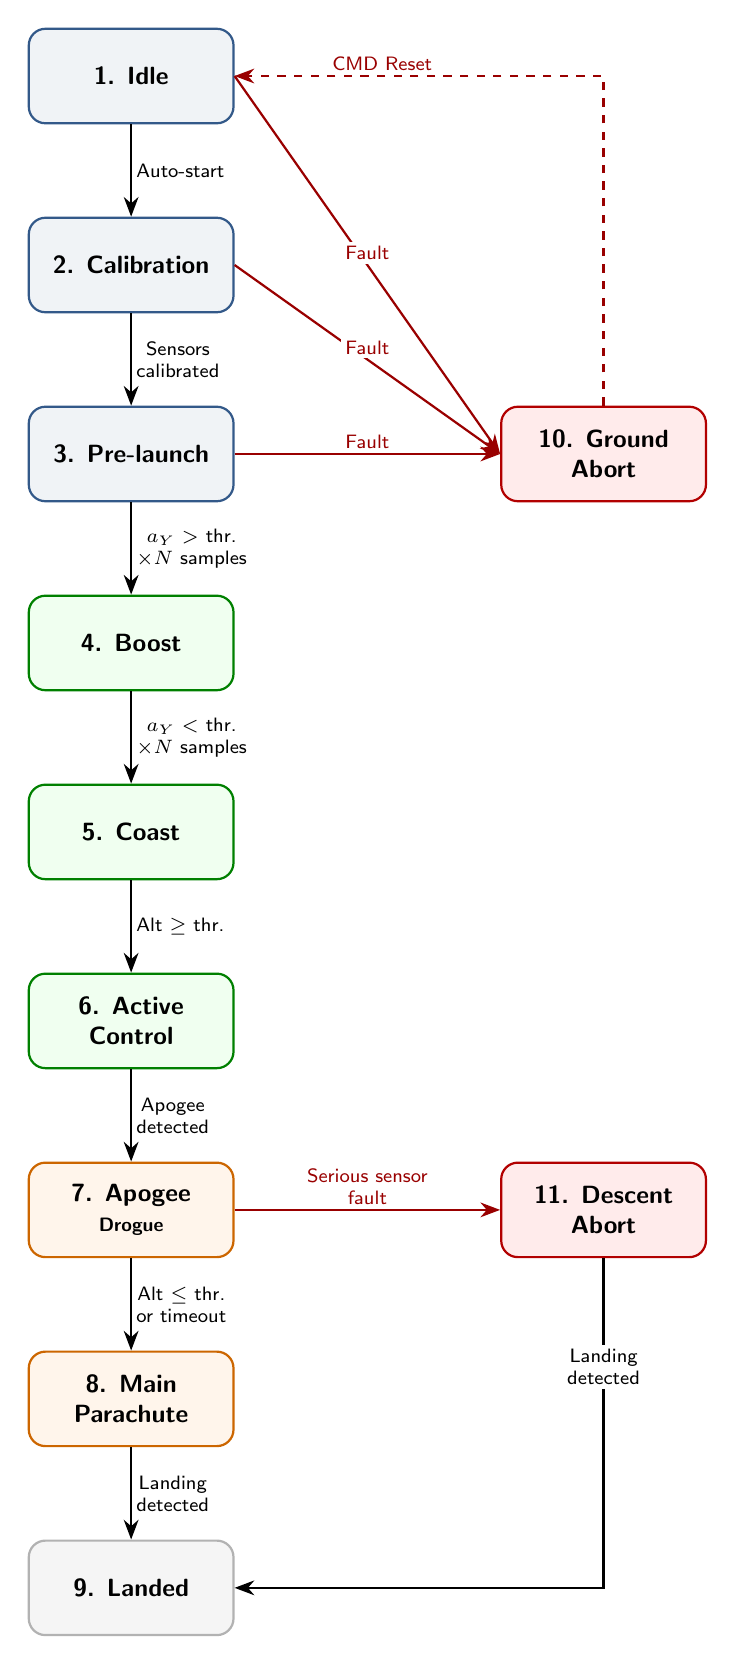
\begin{tikzpicture}[
    state/.style={draw, rounded corners=6pt, thick, minimum width=2.6cm, minimum height=1.2cm, align=center, font=\sffamily\small\bfseries},
    abortst/.style={state, draw=red!70!black, fill=red!8},
    pyrost/.style={state, draw=orange!80!black, fill=orange!8},
    groundst/.style={state, draw=EtseNavy!80, fill=EtseNavy!6},
    flightst/.style={state, draw=green!50!black, fill=green!6},
    terminalst/.style={state, draw=gray!60, fill=gray!8},
    arr/.style={-{Stealth[length=2.5mm]}, thick},
    faultarr/.style={arr, red!60!black},
    cmd/.style={arr, red!60!black, dashed},
    lbl/.style={font=\sffamily\scriptsize, align=center, fill=white, inner sep=1.5pt},
]

% --- Nominal flow: vertical column ---
\node[groundst]   at (0, 0)     (idle)   {1. Idle};
\node[groundst]   at (0, -2.4)  (cal)    {2. Calibration};
\node[groundst]   at (0, -4.8)  (pre)    {3. Pre-launch};
\node[flightst]   at (0, -7.2)  (boost)  {4. Boost};
\node[flightst]   at (0, -9.6)  (coast)  {5. Coast};
\node[flightst]   at (0, -12.0) (actrl)  {6. Active\\Control};
\node[pyrost]     at (0, -14.4) (apogee) {7. Apogee\\{\scriptsize\textit{Drogue}}};
\node[pyrost]     at (0, -16.8) (main)   {8. Main\\Parachute};
\node[terminalst] at (0, -19.2) (landed) {9. Landed};

% --- Abort states (right column) ---
\node[abortst] at (6, -4.8)  (gabort) {10. Ground\\Abort};
\node[abortst] at (6, -14.4) (dabort) {11. Descent\\Abort};

% --- Nominal transitions (black solid, vertical) ---
\draw[arr] (idle)   -- node[lbl, right] {Auto-start} (cal);
\draw[arr] (cal)    -- node[lbl, right] {Sensors\\calibrated} (pre);
\draw[arr] (pre)    -- node[lbl, right] {$a_Y >$ thr.\\$\times N$ samples} (boost);
\draw[arr] (boost)  -- node[lbl, right] {$a_Y <$ thr.\\$\times N$ samples} (coast);
\draw[arr] (coast)  -- node[lbl, right] {Alt $\geq$ thr.} (actrl);
\draw[arr] (actrl)  -- node[lbl, right] {Apogee\\detected} (apogee);
\draw[arr] (apogee) -- node[lbl, right] {Alt $\leq$ thr.\\or timeout} (main);
\draw[arr] (main)   -- node[lbl, right] {Landing\\detected} (landed);

% --- Ground abort (red solid, from ground states to abort) ---
\draw[faultarr] (idle.east)  -- node[lbl, above] {Fault} (gabort.west);
\draw[faultarr] (cal.east)   -- node[lbl, above] {Fault} (gabort.west);
\draw[faultarr] (pre.east)   -- node[lbl, above] {Fault} (gabort.west);

% --- Ground abort reset (dashed, routed back up) ---
\draw[cmd] (gabort.north) |- node[lbl, above, pos=0.8] {CMD Reset} (idle.east);

% --- Descent abort (red solid, from Apogee) ---
\draw[faultarr] (apogee.east) -- node[lbl, above] {Serious sensor\\fault} (dabort.west);

% --- Descent abort to landed (black solid) ---
\draw[arr] (dabort.south) |- node[lbl, above, pos=0.2] {Landing\\detected} (landed.east);

\end{tikzpicture}%
}
\caption{Flight controller state diagram. Black solid arrows: automatic transitions. Red solid arrows: fault-triggered transitions. Red dashed arrows: remote operator command overrides.}
\label{fig:state_machine}
\end{figure}

\paragraph{Ground States}

\textbf{Idle} is the initial state after power-on or reset. On entry, all pyrotechnic channels are disarmed, the calibration context is cleared, and the SD card is mounted and opened for logging. Sensors operate in low-power mode. The transition to \emph{Calibration} occurs automatically after sensor initialization completes when the auto-start flag is enabled (\cfg{AUTO\_START\_CALIBRATION}).

In the \textbf{Calibration} state, SD logging is enabled and all sensors switch to high-performance mode. Three calibration processes execute concurrently:
\begin{itemize}
    \item \textbf{Reference pressure:} The first \cfg{PRESSURE\_CALIBRATION\_DISCARD\_SAMPLES} samples are discarded to allow sensor stabilization; the subsequent \cfg{PRESSURE\_CALIBRATION\_SAMPLES} samples are averaged to establish the ground-level barometric reference.
    \item \textbf{Gyroscope bias:} The first \cfg{GYRO\_CALIBRATION\_DISCARD\_SAMPLES} samples are discarded; the subsequent \cfg{GYRO\_CALIBRATION\_SAMPLES} samples are averaged to determine the zero-rate bias on all three axes.
    \item \textbf{GPS fix:} A valid fix with at least \cfg{GPS\_FIX\_MIN\_SATELLITES} satellite, non-zero position, and non-zero altitude is required.
\end{itemize}
Additionally, the state waits for the onboard Kalman filter to converge before considering calibration complete. The state machine advances to \emph{Pre-launch} only when all three calibrations are simultaneously valid and the filter has converged.

In the \textbf{Pre-launch} state, the rocket is on the launch rail, fully calibrated and awaiting ignition. A confirmation counter is initialized. The transition to \emph{Boost} is triggered when the Y-axis acceleration exceeds the configured threshold (\cfg{PRELAUNCH\_BOOST\_ACCEL\_Y\_THRESHOLD}) for a configurable number of consecutive samples (\cfg{PRELAUNCH\_BOOST\_CONSECUTIVE\_SAMPLES}), indicating motor ignition.

\paragraph{Flight States}

During the \textbf{Boost} state the motor is active and the vehicle experiences sustained positive acceleration. The transition to \emph{Coast} occurs when the measured acceleration drops below the configured threshold (\cfg{BOOST\_COAST\_ACCEL\_Y\_THRESHOLD}) for the required number of consecutive samples (\cfg{BOOST\_COAST\_CONSECUTIVE\_SAMPLES}), indicating motor burnout.

The \textbf{Coast} state represents the unpowered ascent phase after motor burnout. The transition to \emph{Active Control} occurs when the barometric altitude exceeds a configurable height threshold (\cfg{COAST\_ACTIVE\_CONTROL\_BAROM\_ALT\_THRESHOLD}) \req{EuRoC-LV-RQT-0680}.

During the \textbf{Active Control} phase the vehicle is in ascending ballistic flight. The active airbrake control algorithm (detailed in Section~\ref{subsec:active_flight_control}) modulates drag to converge on the target apogee. Multiple apogee detection criteria are monitored redundantly in a logical OR configuration, any single criterion triggers the transition to \emph{Apogee} \req{EuRoC-LV-RQT-0350}. Each criterion can be individually enabled or disabled via its corresponding configuration flag:
\begin{itemize}
    \item Barometric altitude $\geq$ threshold (\cfg{ACTIVE\_CONTROL\_APOGEE\_BAROM\_ALT\_THRESHOLD}).
    \item GPS altitude $\geq$ threshold (\cfg{ACTIVE\_CONTROL\_APOGEE\_GPS\_ALT\_THRESHOLD}).
    \item GPS vertical velocity $\leq$ threshold (\cfg{ACTIVE\_CONTROL\_APOGEE\_GPS\_VEL\_Y\_THRESHOLD}), indicating the onset of descent.
    \item Safety timeout from state entry (\cfg{ACTIVE\_CONTROL\_APOGEE\_DELAY\_MS}, enabled via \cfg{ACTIVE\_CONTROL\_APOGEE\_DELAY\_ENABLED}).
\end{itemize}

\paragraph{Recovery States}

On entry to the \textbf{Apogee} state, the drogue parachute pyrotechnic channel is immediately fired via the Powerboard relay driver (see Section~\ref{subsubsection:avionics_bay}). The transition to \emph{Main Parachute} occurs when either the barometric altitude descends to the configured threshold (\cfg{APOGEE\_MAIN\_PARACHUTE\_BAROM\_ALT\_THRESHOLD}) or the configured timeout elapses (\cfg{APOGEE\_MAIN\_PARACHUTE\_DELAY\_MS}, enabled via \cfg{APOGEE\_MAIN\_PARACHUTE\_DELAY\_ENABLED}).

On entry to the \textbf{Main Parachute} state, the main parachute pyrotechnic channel is fired. Per EuRoC competition rules, the main parachute must not be deployed at an altitude higher than 450\,m AGL \req{EuRoC-LV-RQT-0370}; this limit is enforced through the configurable threshold (\cfg{APOGEE\_MAIN\_PARACHUTE\_BAROM\_ALT\_THRESHOLD}). A landing confirmation counter is initialized. The transition to \emph{Landed} requires both conditions to be satisfied simultaneously for the configured number of consecutive samples (\cfg{MAIN\_PARACHUTE\_LANDED\_CONSECUTIVE\_SAMPLES}):
\begin{itemize}
    \item Barometric altitude $\leq$ threshold (\cfg{MAIN\_PARACHUTE\_LANDED\_BAROM\_ALT\_THRESHOLD}).
    \item Barometric vertical velocity $\leq$ threshold (\cfg{MAIN\_PARACHUTE\_LANDED\_BAROM\_VEL\_Y\_THRESHOLD}).
\end{itemize}

\paragraph{Terminal and Abort States}

On entry to the \textbf{Landed} state, all pyrotechnic channels are disarmed. After the configured delay (\cfg{LANDED\_SD\_STOP\_DELAY\_MS}), SD logging is disabled and the log file is closed to ensure data integrity. The system remains in this state, continuing to transmit telemetry with GPS position data to facilitate localization of the vehicle.

The \textbf{Ground Abort} state is activated by system fault detection (sensor initialization failures or SD card errors) during any ground state. On entry, all pyrotechnic channels are disarmed, SD logging is stopped, and the file is closed. The operator can recover the system from this state by issuing a remote reset command, which forces a return to \emph{Idle}.

The \textbf{Descent Abort} state is entered when a serious sensor fault is detected during descent. Unlike the nominal recovery sequence, this state skips the main parachute deployment, allowing the vehicle to descend under the drogue parachute alone at a higher descent rate. The flight controller can continue to operate on descent with only the barometer if needed. The state monitors barometric altitude and velocity and transitions to \emph{Landed} upon landing detection.

\paragraph{Redundant Flight Computer}

A secondary flight computer, identical in architecture to the primary Baseboard, is connected to the main controller via a 2-pin signalling interface. The redundant computer carries its own independent set of sensors (barometer, IMU, and magnetometer) and runs the same flight state machine software, adapted for the redundant hardware. Both computers have physical access to the active control servos; the signalling interface determines which computer has authority.

The 2-pin interface encodes a 2-bit status word driven by the primary controller. Table~\ref{tab:redundancy_signals} defines the signalling protocol.

\begin{table}[H]
\centering
\caption{Redundant flight computer signalling protocol.}
\label{tab:redundancy_signals}
\begin{tabularx}{\textwidth}{c l X}
\toprule
\textbf{Signal} & \textbf{State} & \textbf{Effect} \\
\midrule
\texttt{11} & Nominal & Primary has servo authority. Redundant computer tracks state independently but does not actuate. \\
\addlinespace
\texttt{00} & Fault / Loss of connection & Handover: redundant computer assumes servo authority and continues the flight autonomously. \\
\bottomrule
\end{tabularx}
\end{table}

Under nominal operation, the primary controller holds both pins high (\texttt{11}). If the primary detects a serious sensor fault or becomes unresponsive (connection loss), the signal defaults to \texttt{00}, triggering automatic handover. The redundant computer, running the state machine independently using its own sensor suite, then assumes active control of the airbrake servos for the remainder of the flight.

Separately, a COTS CATS Vega flight computer (Section~\ref{subsubsection:avionics_bay}) runs its own open-source firmware with independent apogee detection and has dedicated access to the recovery pyrotechnic channels. The CATS Vega must fly the specific firmware version mandated by the EuRoC organization \req{EuRoC-LV-RQT-0450}. It operates fully decoupled from the SRAD flight software and serves as a last-resort recovery backup.

\paragraph{Confirmation Counter Mechanism}

All safety-critical transitions that rely on sensor thresholds employ a consecutive sample confirmation mechanism to prevent false triggers from transient noise or anomalous readings. A condition must be continuously satisfied for $N$ consecutive state machine cycles before the transition fires. If the condition is violated at any point during the count, the counter resets to zero. Table~\ref{tab:confirm_counters} lists all guarded transitions with their corresponding configuration constants.

\begin{table}[H]
\centering
\caption{Confirmation counter parameters for safety-critical transitions.}
\label{tab:confirm_counters}
\small
\begin{tabularx}{\textwidth}{l l X}
\toprule
\textbf{Transition} & \textbf{Samples} & \textbf{Condition} \\
\midrule
Pre-launch $\rightarrow$ Boost
    & \cfg{..\_CONSECUTIVE\_SAMPLES}
    & $a_Y >$ \cfg{PRELAUNCH\_BOOST\_ACCEL\_Y\_THRESHOLD} \\
\addlinespace
Boost $\rightarrow$ Coast
    & \cfg{..\_CONSECUTIVE\_SAMPLES}
    & $a_Y <$ \cfg{BOOST\_COAST\_ACCEL\_Y\_THRESHOLD} \\
\addlinespace
Main Par. $\rightarrow$ Landed
    & \cfg{..\_CONSECUTIVE\_SAMPLES}
    & Alt $\leq$ \cfg{..\_BAROM\_ALT\_THRESHOLD} $\wedge$ $|v| \leq$ \cfg{..\_VEL\_Y\_THRESHOLD} \\
\addlinespace
Descent Ab. $\rightarrow$ Landed
    & \cfg{..\_CONSECUTIVE\_SAMPLES}
    & Alt $\leq$ \cfg{..\_BAROM\_ALT\_THRESHOLD} $\wedge$ $|v| \leq$ \cfg{..\_VEL\_Y\_THRESHOLD} \\
\bottomrule
\end{tabularx}
\end{table}

\paragraph{Remote Command Interface}

The ground station operator can override automatic transitions at any point during the flight via commands transmitted over the LoRa telemetry link. Commands are processed with higher priority than the state handler: if a valid command is received in a given cycle, the corresponding transition is executed without evaluating the current state's handler logic.

\begin{table}[H]
\centering
\caption{Remote operator commands and their effects on the state machine.}
\label{tab:remote_commands}
\begin{tabularx}{\textwidth}{l X}
\toprule
\textbf{Command} & \textbf{Effect} \\
\midrule
Reset & Force return to \emph{Idle} from any state. \\
\bottomrule
\end{tabularx}
\end{table}

\paragraph{Sensor Power Management}

To optimize power consumption, the flight software dynamically reconfigures the sensor operating modes based on the current state. Sensors are placed in low-power idle mode during ground states prior to calibration and after landing or abort, and switched to high-performance mode for the active flight envelope.

\begin{table}[H]
\centering
\caption{Sensor operating mode allocation by flight state.}
\label{tab:sensor_modes}
\begin{tabularx}{\textwidth}{l l X}
\toprule
\textbf{State Range} & \textbf{Sensor Mode} & \textbf{Sampling Timers} \\
\midrule
Idle & Low power (idle) & Stopped \\
Calibration through Main Parachute & High performance & Active (100\,Hz) \\
Landed / Ground Abort / Descent Abort & Low power (idle) & Stopped \\
\bottomrule
\end{tabularx}
\end{table}

\paragraph{Data Logging}

SD card logging is enabled upon entry to the \emph{Calibration} state and remains active through all subsequent flight states until landing or abort. Each state machine cycle produces a 104-byte record containing raw sensor readings, computed state estimates, GPS data, system fault flags, and the current state identifier. Records are enqueued into a FreeRTOS queue and written asynchronously to the SD card by a dedicated logging task in buffers of \cfg{SD\_LOGGING\_RECORDS\_PER\_BUFFER} records, ensuring that file I/O latency does not affect the determinism of the main state machine loop.

% =========================================================================
% 3. MISSION CONCEPT OF OPERATIONS OVERVIEW
% =========================================================================
\section{Mission concept of operations overview} 
% RULE: Mission phases, nominal operation, phase transitions.

\textcolor{red}{Responsable: Angelo. Apoyo: Álvaro Sáez. 1-3 páginas}

\vspace{1cm}

\textcolor{red}{Tomar como base la corrección realizada en el progress report. Revisar requitos de EUROC que hay información acerca de esto a partir del punto 5.}


The Concept of Operations for the launch vehicle is governed by the flight controller's state machine, which is segmented into four primary operational phases: Ground, Ascent, Descent, and Abort. This architecture ensures deterministic behaviour and defines failsafe transitions throughout the mission profile.

\begin{figure}[H]
    \centering
    % Placeholder for the provided state machine diagram
    \includegraphics[width=\textwidth]{state_machine_diagram.png}
    \caption{Avionics state machine diagram detailing nominal flight phases and abort condition transitions.}
    \label{fig:state_machine}
\end{figure}

As illustrated in Figures \ref{fig:state_machine} and \ref{fig:conops_diagram}, nominal operations progress sequentially based on specific telemetry and timing triggers. The transition logic and state actions are detailed in Table \ref{tab:conops_states}.

\begin{figure}[H]
    \centering
    % Placeholder for the provided state machine diagram
    \includegraphics[width=\textwidth]{CONOPS_Diagram.png}
    \caption{NAOS EVO launcher Concept of Operation Diagram}
    \label{fig:conops_diagram}
\end{figure}

\begin{table}[H]
    \centering
    \caption{Flight controller state machine transition logic and nominal phase behaviours.}
    \label{tab:conops_states}
    \begin{tabularx}{\textwidth}{|l|l|X|}
        \hline
        \rowcolor{EtseNavy}
        \textbf{\textcolor{white}{Phase}} & \textbf{\textcolor{white}{State}} & \textbf{\textcolor{white}{Condition \& Behaviour}} \\ \hline
        Ground & IDLE & Pseudo-state initiated upon hardware switch ON. \\ \hline
        \rowcolor{LightGrayTable}
        Ground & INIT & Avionics initialisation sequence. Transitions to CALIBRATION upon receiving the remote GO signal via telemetry. \\ \hline
        Ground & CALIBRATION & Sensor baseline establishment. Transitions to PRELAUNCH once sensors are confirmed calibrated. \\ \hline
        \rowcolor{LightGrayTable}
        Ground & PRELAUNCH & SD logging activation. Awaits IGNITION detection algorithm trigger. \\ \hline
        Ascent & BOOST & Active thrust phase. \\ \hline
        \rowcolor{LightGrayTable}
        Ascent & COASTING & Burn-out. Active control disengaged. Triggered by accelerometer-based motor burn-out detection. \\ \hline
        Ascent & ACTIVE CONTROL & Active control algorithms engaged after passing a predefined altitude constraint. \\ \hline
        \rowcolor{LightGrayTable}
        Descent & APOGEE & Drogue parachute deployment, triggered by barometric and inertial apogee detect  ion. \\ \hline
        Descent & MAIN PARACHUTE & Main parachute deployment, triggered by a secondary descent altitude constraint. \\ \hline
        \rowcolor{LightGrayTable}
        Descent & LANDED & Touchdown detection. Disables non-essential sensors and high-current draw systems to preserve battery life for recovery telemetry. \\ \hline
    \end{tabularx}
\end{table}

Anomalies detected in telemetry or control loops force an immediate transition to the respective Abort state. A \textbf{Ground Abort} halts the launch sequence. A \textbf{Descent Abort} overrides nominal altitude logic to force immediate parachute deployment, ensuring the vehicle returns within range limits at a safe velocity.
\textbf{Ascent Abort} states are omitted as the rocket will continue its ballistic path and transition to the respective descent states.

\vspace{0.5cm}
\noindent\textbf{Keywords:} main logic for arming/ignition/stage separation/deployment events, trajectories, influence of wind, propulsion thrust curve, predicted apogee, aerodynamic stability, centre of gravity, centre of pressure, velocity, acceleration, descent rates.

% =========================================================================
% 4. CONCLUSIONS AND OUTLOOK
% =========================================================================
\section{Conclusions and outlook} \textcolor{red}{Responsable:JD. 1-3 páginas}
% RULE: Summary of achievements, reflections, project outcomes, lessons learned, remaining challenges.

\vspace{0.5cm}
\noindent\textbf{Keywords:} achievements, reflections, project outcomes, lessons learned, way forward, remaining design challenges, areas for improvement.

\newpage
% %%%%%%%%%%%%%%%%%%%%%%%%%%%%%%%%%%%%%%%%%%%%%%%%%%%%%%%%%%%%%%%%%%%%%%%%%
% WARNING: MAXIMUM 50 PAGES UNTIL HERE (Excluding figures, etc.)
% %%%%%%%%%%%%%%%%%%%%%%%%%%%%%%%%%%%%%%%%%%%%%%%%%%%%%%%%%%%%%%%%%%%%%%%%%
\vspace*{5cm}
\begin{center}
    \Huge \textbf{\textcolor{EtseNavy}{--- MAXIMUM 50 PAGES UNTIL HERE ---}} \\
    \vspace{1cm}
    \Large \textit{Any content past this point belongs to the Appendices and does not count towards the page limit.}
\end{center}
\newpage

% =========================================================================
% 5. APPENDICES (MANDATORY ORDER)
% =========================================================================
\section{Appendices}

\subsection{System data} \textcolor{red}{Responsable: Miguel Rodríguez. Apoyo: Gonzalo, Mateo}

\vspace{1cm}

\textcolor{red}{Revisar formato del progress report, cosas que se nos puedan escapar, y actualizados los datos. Performance Mateo. OJO, se explica todo con tablas.}
% RULE: Vehicle/system weights, measures, performance data in tabular manner.

\subsection{Detailed test reports} \textcolor{red}{Aquí hay que brillar u decir todo lo que hemos estado haciendo}
% RULE: Must follow this EXACT order. If a report is not applicable, the team must include a page marked "THIS PAGE INTENTIONALLY LEFT BLANK" in its place.

\subsubsection{Ground test demonstration of recovery system} \textcolor{red}{Responsable: Paula}
% INTEGRATION NOTE: Recovery deployment test details go here.

\subsubsection{Wind tunnel experiments} \textcolor{red}{Responsable: Paula.}
% INTEGRATION NOTE: If no flight test was performed, we can put the blank page here, or detail a sub-scale flight test if available. 

\subsubsection{Electronics thermal testing} \textcolor{red}{Responsable: Jose Reyes/Alejandro Ariza}
% INTEGRATION NOTE: Avionics thermal validation details.

\subsubsection{Static hot-fire test (SRAD)} \textcolor{red}{Responsable: Jesús}
% INTEGRATION NOTE: APCP 6-Bates static fire results, thrust/pressure curves.

\vspace{1cm}

\textcolor{red}{Páginas 21 y 22 que se vean claras las leyendas y no den pie a confusión. Actualizar si es posible con nuevas curvas.}

% -------------------------------------------------------------------------
% N/A SECTION: Hybrid/liquid loading
% -------------------------------------------------------------------------
\subsubsection{Hybrid/liquid propellant loading and offloading test (SRAD)}
\vspace*{\fill}
\begin{center}
    \textbf{THIS PAGE INTENTIONALLY LEFT BLANK} \\
    \vspace{0.5cm}
    \textit{(Not applicable: The NAOS EVO launch vehicle utilises a solid propellant motor.)}
\end{center}
\vspace*{\fill}
\newpage

\subsubsection{Combustion chamber pressure test (SRAD)} \textcolor{red}{Responsable: Pablo (propulsión). Apoyo: Jesús.}
% INTEGRATION NOTE: The Hydrostatic/Hydraulic pressure test for the AISI 304 casing.

A hydrostatic proof pressure test was performed on the SRAD stainless-steel combustion chamber flight article (CC-01) to verify its structural integrity and demonstrate compliance with the EuRoC requirements for SRAD pressure vessels. The test was conducted in accordance with \req{EuRoC-LV-RQT-0640}, which requires the intended flight article to successfully withstand a proof pressure corresponding to 1.5 times the Maximum Expected Operating Pressure (MEOP), without significant anomalies, for at least twice the maximum expected system working time.\\

The test article was connected to an HBM 10T manual hydraulic pump (BH-01) through a Hidraflex 1/4” BSP male to 1/2” BSP female adapter (AD-01) and an SRAD stainless-steel nozzle plug (TP-01). ISO 46 hydraulic oil (AC-01) was used as the test fluid. Two independent pressure sensors (PS-01 and PS-02) were connected to a Dewesoft X data acquisition system (DAQ-01) to continuously monitor and record the pressure throughout the test. Two cameras (CAM-01 and CAM-02) were also used to provide visual evidence of the pressurization and pressure-holding phases. Personnel were protected by a concrete blast shield (BS-01).

% \begin{figure}[H]
%     \centering
%     \includegraphics[width=1\textwidth]{hyd}
%     \caption{Empirical thrust (kg) and chamber pressure (bar/atm) curves versus time (s) recorded during static fire testing.}
%     \label{fig:thrust_pressure_curves}
% \end{figure}

\begin{figure}[H]
    \centering
    \begin{subfigure}[b]{0.65\textwidth}
        \centering
        \includegraphics[width=\textwidth]{propulsion/hyd_test1.png}
        \caption{Motor prepared with the pump and the pressure sensors connected and ready to begin with the test}
        \label{fig:motor_hyd_test}
    \end{subfigure}
    \hfill
    \begin{subfigure}[b]{0.34\textwidth}
        \centering
        \includegraphics[width=\textwidth]{propulsion/hyd_test3.png}
        \caption{Oil pump with analogic measure and the camera to register the data from the pump sensor}
        \label{fig:oil_pump}
    \end{subfigure}
    %\caption{Rendimiento de la hélice en función de $C_p$ y $J$}
    \label{fig:motor_hyd_test}
\end{figure}

Prior to pressurization, the combustion chamber and nozzle plug were visually inspected and the test assembly was installed and connected. The chamber was completely filled with hydraulic oil, taking care to remove trapped air from the system before tightening the connection. Both pressure sensors and the cameras were then verified and positioned for data acquisition and visual monitoring. Pressurization was performed progressively, in approximately 10 bar increments, with pauses at each increment to inspect the system for leakage.

\begin{figure}[H]
    \centering
    \includegraphics[width=0.25\textwidth]{propulsion/hyd_test2.png}
    \caption{Motor being filled with oil}
    \label{fig:filling_oil}
\end{figure}

The initial proof pressure target was 105 bar. This pressure was successfully reached and maintained for the required holding period without evidence of leakage, abnormal pressure decay, or structural anomalies. Following the successful completion of the planned test stage, the pressure was further increased for additional verification. A maximum pressure of 108 bar was subsequently achieved and maintained for more than 30 seconds, with good agreement between PS-01 and PS-02 throughout the test.

\begin{figure}[H]
    \centering
    \begin{subfigure}[b]{0.75\textwidth}
        \centering
        \includegraphics[width=\textwidth]{propulsion/hyd_test_pressure.png}
        \caption{}
        \label{fig:hyd_pressure1}
    \end{subfigure}
    \hfill
    \begin{subfigure}[b]{0.75\textwidth}
        \centering
        \includegraphics[width=\textwidth]{propulsion/hyd_test_pressure2.png}
        \caption{}
        \label{fig:oil_pump}
    \end{subfigure}
    \caption{pressure measurements during the test}
    \label{fig:hyd_measurements}
\end{figure}

After controlled depressurization, the combustion chamber, nozzle plug, adapter, threaded interfaces, sealing surfaces, fasteners, and other critical areas were visually inspected. No visible deformation, cracks, leaks, or other structural anomalies were identified, and no evidence of damage or degradation was observed. The maximum pressure achieved, 108 bar, corresponded to more than 1.5 times the chamber MEOP, thereby satisfying the applicable EuRoC proof pressure requirement.

The test therefore successfully demonstrated the structural integrity of the intended flight combustion chamber and provided additional confidence in its structural margin. The use of two independent pressure sensors also enabled cross-validation of the recorded pressure data. No major corrective actions were identified, and the combustion chamber was considered ready for subsequent qualification and flight activities.


% -------------------------------------------------------------------------
% N/A SECTION: Proof pressure vessels
% -------------------------------------------------------------------------
\subsubsection{Proof pressure testing pressure vessels (SRAD, Modified COTS)}
\vspace*{\fill}
\begin{center}
    \textbf{THIS PAGE INTENTIONALLY LEFT BLANK} \\
    \vspace{0.5cm}
    \textit{(Not applicable: The solid propulsion architecture does not incorporate pressurized fluid vessels.)}
\end{center}
\vspace*{\fill}
\newpage

% -------------------------------------------------------------------------
% N/A SECTION: Burst pressure vessels
% -------------------------------------------------------------------------
\subsubsection{Burst pressure testing pressure vessels (SRAD, Modified COTS)}
\vspace*{\fill}
\begin{center}
    \textbf{THIS PAGE INTENTIONALLY LEFT BLANK} \\
    \vspace{0.5cm}
    \textit{(Not applicable: The solid propulsion architecture does not incorporate pressurized fluid vessels.)}
\end{center}
\vspace*{\fill}
\newpage

\subsubsection{Test of SRAD flight computers with capability of actuating the recovery systems}
% INTEGRATION NOTE: HIL tests, galvanic isolation verification, relay actuation tests.

\subsection{Hazard analysis report} \textcolor{red}{Responsable: }

\vspace{1cm}

\textcolor{red}{Tomar como base el progress report con las correcciones de los jueces, si hicieron comentarios}

\subsection{Risk assessment} \textcolor{red}{Responsable: Álvaro Sáez}
% RULE: FMECA Matrix. Likelihood, Severity, Criticality Ranking.
% INTEGRATION NOTE: We will expand the Failure Modes for Recovery here as requested in the meeting.

\subsection{Compliance matrix} \textcolor{red}{Responsable: Miguel Tejera. Apoyo: Miguel Rodríguez.}
% RULE: SRD requirements and team compliance (Fully, Partially, Non-compliant, N/A).

\subsection{Checklists} \textcolor{red}{Responsable: JD}
% RULE: Assembly, pre-flight, and launch operations. Off-nominal alternate flows.
% INTEGRATION NOTE: Onboard cameras MUST BE REMOVED from these checklists.

\subsection{Launch support equipment} 

With the aim of ensuring operational safety, regulatory compliance, and seamless execution during field activities, a dedicated Launch Support Equipment matrix has been established. Table~\ref{tab:launch_support_equipment} summarizes the essential items, tools, and consumables allocated across each subsystem—from ignition control and telemetry tracking to mechanical assembly and range safety gear—required on-site throughout the assembly, arming, and launch phases.
\subsubsection{Launch support equipment list} 

% Required packages in your preamble:
% \usepackage{longtable}
% \usepackage{booktabs}

\begin{longtable}{p{0.65\textwidth} p{0.3\textwidth}}
\caption{Launch Support Equipment Inventory} \label{tab:launch_support_equipment} \\
\toprule
\textbf{Item / Equipment} & \textbf{Quantity} \\
\midrule
\endfirsthead

\multicolumn{2}{c}{\tablename\ \thetable\ -- \textit{Continued from previous page}} \\
\toprule
\textbf{Item / Equipment} & \textbf{Quantity} \\
\midrule
\endhead

\midrule
\multicolumn{2}{r}{\textit{Continued on next page...}} \\
\endfoot

\bottomrule
\endlastfoot

% -------------------------------------------------------------
\multicolumn{2}{l}{\textbf{1. Launch Control \& Ignition Subsystem (LCS \& Propulsion GSE)}} \\
\midrule
Physical Ignition Control Box & 1 \\
Igniter Cable & 1 line \\
Pyrotechnic Motor Igniter & 2 \\
Ignition Battery Pack (Battery+Connectors) & 1 \\
Nozzle Throat Depth Alignment Gauge & 1 \\
Thermal-Resistant Adhesive Tape & 1 roll \\
Sun Thermal Protectors & 1 set \\
\midrule

% -------------------------------------------------------------
\multicolumn{2}{l}{\textbf{2. Avionics, Telemetry \& Ground Station (Ground Station \& Avionics GSE)}} \\
\midrule
Ground Station Terminal (Laptop) (LCC Station) & 1 primary \\
GS Tracking Antennas & 2 antennas \\
\midrule

% -------------------------------------------------------------
\multicolumn{2}{l}{\textbf{3. Field Toolkit, Fasteners \& Servicing Tools (Field Tools)}} \\
\midrule
Heavy Mechanics Toolset (Mannesmann Box) & 1 complete case \\
Allen Key Kit & 1 full set \\
Precision Screwdriver Kit & 1 set \\
Dedicated Flathead Screwdriver for Fin Mounting & 1 \\
Pliers \& Wire Cutters & 2 pairs \\
Heavy-Duty Scissors & 1 \\
Digital Multimeter (DMM) with Probes & 1 unit \\
Step Ladder & 1 unit \\
Sledgehammer & 1 \\
Standard Claw Hammer & 1 \\
Shovel & 1 \\
Pickaxe & 1 \\
Utility Knife & 1 \\
Metal Bastard File & 1 \\
Gas Blowtorch & 1 mini blowtorch \\
Lighters & 2 \\
PVC Spring Tensioning Jig Tube & 1 tool \\
M3 Screws Box & 1 compartment box \\
\midrule

% -------------------------------------------------------------
\multicolumn{2}{l}{\textbf{4. Field Consumables, Tapes, Fasteners \& Chemicals}} \\
\midrule
High-Temperature Aluminum Adhesive Foil Tape & 2 rolls \\
Masking Tape & 2 rolls \\
High-Grade Electrical Insulating Tape & 2 rolls \\
Assorted Heavy-Duty Cable Ties & 1 pack \\
Vent Hole Masking Pre-Flight Stickers & 1 sheet \\
Mechanical Lubricating Grease & 1 tub \\
Stainless Steel Safety Tie Wire & 1 roll \\
Utility Rigging Rope & 1 spool \\
Abrasive Sandpaper Sheets & 3 sheets \\
Assorted Fasteners \& Hardware Organizer Box & 1 organizer case \\
\midrule

% -------------------------------------------------------------
\multicolumn{2}{l}{\textbf{5. Range Safety, PPE \& Field Administration}} \\
\midrule
Fire Extinguisher & 1 certified unit \\
Heavy-Duty Mechanical Work Gloves & 5 pairs \\
Safety Glasses & 5 pairs \\
Walkie-Talkies & 4 units \\
Hardcover Field Clipboard & 1 \\
Permanent Pens & 4 \\

\end{longtable}

\subsubsection{Launch support equipment simple operational manual} \textcolor{red}{ NA}
\subsubsection{Launch support equipment details} \textcolor{red}{NA}
\paragraph{5.7.3.1. Detailed structural and mechanical calculation}
\paragraph{5.7.3.2. Detailed logical process diagrams}
\paragraph{5.7.3.3. Detailed software architecture} 
\paragraph{5.7.3.4. Detailed electrical architecture}
\label{para:detailed_electrical_architecture}

Figure~\ref{fig:electrical_connection_diagram} illustrates the overall electrical integration, isolated power domains, inter-board communication buses, and pad safety arming interlocks of the NAOS EVO avionics subsystem.

The hardware interfaces are categorized into three physical interconnection types:
\begin{itemize}
    \item \textbf{Soldered Connections (Cyan Lines):} Vibration-resistant, surface-mounted sensors and non-volatile storage connected directly to their MCUs. The primary STM32 MCU drives the sensor suite (BMP581, IIM-42653, LSM6DSV32, IIS2MDCTR) and SD/Flash memory. The Active Control Redundancy PCB incorporates its own soldered sensor suite (LSM6DSV32, BMP581, IIS2MDCTR).
    \item \textbf{Cabled Interconnects (Gray Lines):} Wiring harnesses routing power and control signals across modular units. The Powerboard supplies the primary STM32 MCU, RunCam Split 4 camera, active control servo, and pyrotechnic deployment channels.
    \item \textbf{Communication Bus (Green Dashed Line):} Multi-node digital bus interconnecting the STM32 MCU, Redundant Active Control PCB, and Telemetry \& GNSS computer for state synchronization, error status propagation, and control authority handoff.
\end{itemize}

\textbf{Power Domain Isolation and Arming Safety:} Electrical power is strictly partitioned into four isolated domains (Powerboard, Active Control Redundancy, CATS Vega Recovery, and Telemetry \& GNSS Computer), each powered by an independent $2500\,\text{mAh}$ $2\text{S}$ Li-Ion battery pack with its own Remove-Before-Flight (RBF) pull-pin switch. 

Pyrotechnic launchpad safety is enforced via a mechanical \textbf{Pull Pin (Arming)} interlock interrupting the firing channels for both Pyro 1 (Drogue Chute / $\text{CO}_2$) and Pyro 2 (Main Chute / Tender Desc), ensuring ejection charges cannot energize until fully armed on the rail.

\begin{figure}[H]
    \centering
    \includegraphics[width=0.85\textwidth]{Conection diagram.png}
    \caption{Complete electrical connection diagram and power topology of the NAOS EVO avionics subsystem.}
    \label{fig:electrical_connection_diagram}
\end{figure}

\paragraph{5.7.3.5. Detailed hydraulic/fluid architecture} \textcolor{red}{NA}

\subsection{Engineering drawings}
% RULE: Revision controlled technical drawings.

\subsection{Subsystem details (optional)}

\subsubsection{Error-State Kalman Filter (ESKF) Derivation}

\paragraph{State Definition and IMU Propagation:}
The ESKF distinguishes between the nominal state ($\mathbf{x}$) and the error state ($\delta\mathbf{x}$). The nominal state is defined by position, velocity, and attitude quaternion in the North-East-Down (NED) frame:
\[
\mathbf{x} = \begin{bmatrix} \mathbf{r}_{NED} \\ \mathbf{v}_{NED} \\ \mathbf{q}_{B \leftarrow NED} \end{bmatrix}
\]

The error state encompasses the small deviations, where attitude error is represented by a minimal 3-parameter rotation vector $\delta\boldsymbol{\theta}$:
\[
\delta\mathbf{x} = \begin{bmatrix} \delta\mathbf{r}_{NED} \\ \delta\mathbf{v}_{NED} \\ \delta\boldsymbol{\theta} \end{bmatrix}
\]

The nominal state is propagated forward in time using the Inertial Measurement Unit (IMU) as the control input $\mathbf{u} = [\mathbf{a}_B, \boldsymbol{\omega}_B]^T$, effectively acting as the system's dynamic model. The continuous-time propagation kinematics are:
\[
\dot{\mathbf{r}}_{NED} = \mathbf{v}_{NED}
\]
\[
\dot{\mathbf{v}}_{NED} = DCM_{NED \leftarrow B} \mathbf{a}_B + \mathbf{g}_{NED}
\]
\[
\dot{\mathbf{q}}_{B \leftarrow NED} = \frac{1}{2} \mathbf{q}_{B \leftarrow NED} \otimes \begin{bmatrix} 0 \\ \boldsymbol{\omega}_B \end{bmatrix}
\]

\paragraph{Error-State Kinematics and Covariance Propagation:}
To propagate the covariance matrix $P$, we must linearize the error-state dynamics to find the continuous-time system Jacobian $A = \frac{\partial \mathbf{f}}{\partial \delta\mathbf{x}}$. Evaluating the partial derivatives yields:
\[
A = \begin{bmatrix} 
0_{3\times3} & I_{3\times3} & 0_{3\times3} \\ 
0_{3\times3} & 0_{3\times3} & -DCM_{NED \leftarrow B} [\mathbf{a}_B \times] \\ 
0_{3\times3} & 0_{3\times3} & -[\boldsymbol{\omega}_B \times] 
\end{bmatrix}
\]

This continuous-time Jacobian is discretized over the sampling interval $h = t_k - t_{k-1}$ to form the discrete State Transition Matrix ($F_k$) using a Taylor series expansion approximation:
\[
F_k \approx I + A h + \frac{A^2 h^2}{2}
\]

The error-state covariance matrix $P$ is then propagated to the next time step (a priori estimate):
\[
P_k^- = F_k P_{k-1}^+ F_k^T + Q
\]

\paragraph{Noise Matrices ($Q$ and $R$):}
The process noise covariance matrix $Q$ and measurement noise covariance matrix $R$ quantify the uncertainty in the models and sensors:
\begin{itemize}
    \item \textbf{$Q$ Matrix}: Represents the uncertainty injected during IMU propagation. The diagonal values are derived from the IMU datasheet's continuous noise density parameters (e.g., Velocity Random Walk for accelerometers in $(\text{m/s})/\sqrt{\text{hr}}$, and Angular Random Walk for gyroscopes in $\text{deg}/\sqrt{\text{hr}}$). These continuous parameters are squared to form variances and scaled by the sampling time $\Delta t$ to transition into discrete-time variances.
    \item \textbf{$R$ Matrix}: Represents the uncertainty of the external measurements. The diagonal elements correspond to the variance ($\sigma^2$) of the respective sensors (magnetometer and barometer), determined by analyzing the Root Mean Square (RMS) noise specifications via static statistical calibration.
\end{itemize}

\paragraph{Measurement Updates:}
When a sensor provides a new measurement $\mathbf{z}_k$, the error state is updated by calculating the residual $\mathbf{y}_k = \mathbf{z}_k - \mathbf{h}(\mathbf{x}_k^-)$ and applying the Kalman Gain $K_k$:
\[
K_k = P_k^- H_k^T (H_k P_k^- H_k^T + R_k)^{-1}
\]
\[
\delta\mathbf{x}_k^+ = K_k \mathbf{y}_k
\]

The nominal state is then updated using the composition operator (standard addition for translation, quaternion multiplication for attitude):
\[
\mathbf{x}_k^+ = \mathbf{x}_k^- \oplus \delta\mathbf{x}_k^+
\]

Finally, the error-state covariance is updated to reflect the newly incorporated information:
\[
P_k^+ = (I - K_k H_k) P_k^-
\]

\paragraph{Magnetometer Measurement Function and Jacobian:}
The magnetometer measures the local Earth magnetic field vector in the body frame ($\mathbf{B}_B$). We map the known reference magnetic field from the NED frame ($\mathbf{B}_{NED}$) to the Body frame:
\[
\mathbf{B}_B = DCM_{B \leftarrow NED} \mathbf{B}_{NED}
\]

Accounting for the error state mapping $\mathbf{B}_B = DCM_{B \leftarrow NED} (I - [\delta\boldsymbol{\theta} \times]) \mathbf{B}_{NED}$, the measurement Jacobian $H_{mag} = \frac{\partial \mathbf{h}_{mag}}{\partial \delta\mathbf{x}}$ becomes:
\[
H_{mag} = \begin{bmatrix} 0_{3\times3} & 0_{3\times3} & [DCM_{B \leftarrow NED} \mathbf{B}_{NED} \times] \end{bmatrix}
\]

\paragraph{Barometer Measurement Function and Jacobian:}
The barometer measures ambient pressure $p$ to derive relative altitude $h_{baro}$ above a ground datum $p_0$:
\[
h_{baro} = \left(\left(\frac{p}{p_0}\right)^{\frac{1}{5.256}} - 1\right)\frac{T_0 + 273.15}{L}
\]

Where $L = -0.0065 K/m$ and $T_0 = 15 C$. In the NED frame, the Down component ($r_D$) represents negative altitude. Therefore, the measurement model mapping the nominal state to the barometer observation is $h(\mathbf{x}) = -r_{NED, D}$.

The corresponding $1 \times 9$ measurement Jacobian $H_{baro} = \frac{\partial h_{baro}}{\partial \delta\mathbf{x}}$ directly targets the Z-axis (Down) component of the position error state:
\[
H_{baro} = \begin{bmatrix} 0 & 0 & -1 & 0_{1\times3} & 0_{1\times3} \end{bmatrix}
\]

\subsubsection{Derivation of Algebraic Apogee Altitude Prediction}

To derive the apogee altitude, we begin with Newton's Second Law of Motion for a projectile in unpowered vertical ascent. The two forces acting on the body are gravity and aerodynamic drag, both of which act downwards (in the negative $z$ direction) opposing the upward velocity $v_z$. 

The equation of motion is:
\begin{equation}
    m \frac{dv_z}{dt} = -mg - F_D
\end{equation}

Where the aerodynamic drag force $F_D$ is defined as:
\begin{equation}
    F_D = \frac{1}{2} \rho S_{REF} C_D v_z^2
\end{equation}

Substituting the drag force into the equation of motion yields:
\begin{equation}
    m \frac{dv_z}{dt} = -mg - \frac{1}{2} \rho S_{REF} C_D v_z^2
\end{equation}

Since we want to find the apogee altitude as a function of distance rather than time, we can apply the chain rule to the acceleration term to relate velocity directly to altitude $z$:
\begin{equation}
    \frac{dv_z}{dt} = \frac{dv_z}{dz} \frac{dz}{dt} = v_z \frac{dv_z}{dz}
\end{equation}

Substituting this into the equation of motion gives:
\begin{equation}
    m v_z \frac{dv_z}{dz} = -mg - \frac{1}{2} \rho S_{REF} C_D v_z^2
\end{equation}

Next, we separate the variables $v_z$ and $z$ to prepare for integration:
\begin{equation}
    dz = \frac{m v_z}{-mg - \frac{1}{2} \rho S_{REF} C_D v_z^2} dv_z
\end{equation}

We integrate both sides from the initial state (altitude $z_0$, velocity $v_{z0}$) to the apogee state. At apogee, the altitude is $h_{apogee}$ and the vertical velocity is zero ($0$):
\begin{equation}
    \int_{z_0}^{h_{apogee}} dz = \int_{v_{z0}}^{0} \frac{m v_z}{-mg - \frac{1}{2} \rho S_{REF} C_D v_z^2} dv_z
\end{equation}

The left side evaluates simply to $h_{apogee} - z_0$. For the right side, we can factor out a negative sign and perform a $u$-substitution. Let $u = mg + \frac{1}{2} \rho S_{REF} C_D v_z^2$. The differential is $du = \rho S_{REF} C_D v_z dv_z$, which means $v_z dv_z = \frac{du}{\rho S_{REF} C_D}$. 

Applying this substitution, the integral evaluates to a natural logarithm:
\begin{equation}
    h_{apogee} - z_0 = -\frac{m}{\rho S_{REF} C_D} \left[ \ln \left( mg + \frac{1}{2} \rho S_{REF} C_D v_z^2 \right) \right]_{v_{z0}}^{0}
\end{equation}

Evaluating at the bounds (from $v_{z0}$ to $0$):
\begin{equation}
    h_{apogee} - z_0 = -\frac{m}{\rho S_{REF} C_D} \left( \ln(mg) - \ln \left( mg + \frac{1}{2} \rho S_{REF} C_D v_{z0}^2 \right) \right)
\end{equation}

Finally, some algebraic manipulation gives the completed derived equation for the apogee altitude:
\begin{equation}
    h_{apogee} = z_0 + \frac{m}{\rho S_{REF} C_D} \ln \left( 1 + \frac{v_{z0}^2 \rho S_{REF} C_D}{2mg} \right)
\end{equation}


This redundant architecture was specifically implemented to comply with \req{EuRoC-LV-RQT-0250}, ensuring dual-fault tolerance across all recovery ignition lines.

\end{document}